\documentclass[twoside]{book}

% Packages required by doxygen
\usepackage{fixltx2e}
\usepackage{calc}
\usepackage{doxygen}
\usepackage[export]{adjustbox} % also loads graphicx
\usepackage{graphicx}
\usepackage[utf8]{inputenc}
\usepackage{makeidx}
\usepackage{multicol}
\usepackage{multirow}
\PassOptionsToPackage{warn}{textcomp}
\usepackage{textcomp}
\usepackage[nointegrals]{wasysym}
\usepackage[table]{xcolor}

% Font selection
\usepackage[T1]{fontenc}
\usepackage[scaled=.90]{helvet}
\usepackage{courier}
\usepackage{amssymb}
\usepackage{sectsty}
\renewcommand{\familydefault}{\sfdefault}
\allsectionsfont{%
  \fontseries{bc}\selectfont%
  \color{darkgray}%
}
\renewcommand{\DoxyLabelFont}{%
  \fontseries{bc}\selectfont%
  \color{darkgray}%
}
\newcommand{\+}{\discretionary{\mbox{\scriptsize$\hookleftarrow$}}{}{}}

% Page & text layout
\usepackage{geometry}
\geometry{%
  a4paper,%
  top=2.5cm,%
  bottom=2.5cm,%
  left=2.5cm,%
  right=2.5cm%
}
\tolerance=750
\hfuzz=15pt
\hbadness=750
\setlength{\emergencystretch}{15pt}
\setlength{\parindent}{0cm}
\setlength{\parskip}{3ex plus 2ex minus 2ex}
\makeatletter
\renewcommand{\paragraph}{%
  \@startsection{paragraph}{4}{0ex}{-1.0ex}{1.0ex}{%
    \normalfont\normalsize\bfseries\SS@parafont%
  }%
}
\renewcommand{\subparagraph}{%
  \@startsection{subparagraph}{5}{0ex}{-1.0ex}{1.0ex}{%
    \normalfont\normalsize\bfseries\SS@subparafont%
  }%
}
\makeatother

% Headers & footers
\usepackage{fancyhdr}
\pagestyle{fancyplain}
\fancyhead[LE]{\fancyplain{}{\bfseries\thepage}}
\fancyhead[CE]{\fancyplain{}{}}
\fancyhead[RE]{\fancyplain{}{\bfseries\leftmark}}
\fancyhead[LO]{\fancyplain{}{\bfseries\rightmark}}
\fancyhead[CO]{\fancyplain{}{}}
\fancyhead[RO]{\fancyplain{}{\bfseries\thepage}}
\fancyfoot[LE]{\fancyplain{}{}}
\fancyfoot[CE]{\fancyplain{}{}}
\fancyfoot[RE]{\fancyplain{}{\bfseries\scriptsize Generated by Doxygen }}
\fancyfoot[LO]{\fancyplain{}{\bfseries\scriptsize Generated by Doxygen }}
\fancyfoot[CO]{\fancyplain{}{}}
\fancyfoot[RO]{\fancyplain{}{}}
\renewcommand{\footrulewidth}{0.4pt}
\renewcommand{\chaptermark}[1]{%
  \markboth{#1}{}%
}
\renewcommand{\sectionmark}[1]{%
  \markright{\thesection\ #1}%
}

% Indices & bibliography
\usepackage{natbib}
\usepackage[titles]{tocloft}
\setcounter{tocdepth}{3}
\setcounter{secnumdepth}{5}
\makeindex

% Hyperlinks (required, but should be loaded last)
\usepackage{ifpdf}
\ifpdf
  \usepackage[pdftex,pagebackref=true]{hyperref}
\else
  \usepackage[ps2pdf,pagebackref=true]{hyperref}
\fi
\hypersetup{%
  colorlinks=true,%
  linkcolor=blue,%
  citecolor=blue,%
  unicode%
}

% Custom commands
\newcommand{\clearemptydoublepage}{%
  \newpage{\pagestyle{empty}\cleardoublepage}%
}

\usepackage{caption}
\captionsetup{labelsep=space,justification=centering,font={bf},singlelinecheck=off,skip=4pt,position=top}

%===== C O N T E N T S =====

\begin{document}

% Titlepage & ToC
\hypersetup{pageanchor=false,
             bookmarksnumbered=true,
             pdfencoding=unicode
            }
\pagenumbering{alph}
\begin{titlepage}
\vspace*{7cm}
\begin{center}%
{\Large P\+ID plotter component \\[1ex]\large 1.\+0 }\\
\vspace*{1cm}
{\large Generated by Doxygen 1.8.13}\\
\end{center}
\end{titlepage}
\clearemptydoublepage
\pagenumbering{roman}
\tableofcontents
\clearemptydoublepage
\pagenumbering{arabic}
\hypersetup{pageanchor=true}

%--- Begin generated contents ---
\chapter{E\+S\+P-\/\+I\+DF template app}
\label{index}\hypertarget{index}{}This is a template application to be used with \href{https://github.com/espressif/esp-idf}{\tt Espressif IoT Development Framework}.

Please check \href{https://docs.espressif.com/projects/esp-idf/en/latest/get-started/index.html}{\tt E\+S\+P-\/\+I\+DF docs} for getting started instructions.

{\itshape Code in this repository is in the Public Domain (or C\+C0 licensed, at your option.) Unless required by applicable law or agreed to in writing, this software is distributed on an \char`\"{}\+A\+S I\+S\char`\"{} B\+A\+S\+IS, W\+I\+T\+H\+O\+UT W\+A\+R\+R\+A\+N\+T\+I\+ES OR C\+O\+N\+D\+I\+T\+I\+O\+NS OF A\+NY K\+I\+ND, either express or implied.} 
\chapter{Class Index}
\section{Class List}
Here are the classes, structs, unions and interfaces with brief descriptions\+:\begin{DoxyCompactList}
\item\contentsline{section}{\hyperlink{structnetwork__data}{network\+\_\+data} }{\pageref{structnetwork__data}}{}
\item\contentsline{section}{\hyperlink{structtcp__network__data}{tcp\+\_\+network\+\_\+data} }{\pageref{structtcp__network__data}}{}
\end{DoxyCompactList}

\chapter{File Index}
\section{File List}
Here is a list of all files with brief descriptions\+:\begin{DoxyCompactList}
\item\contentsline{section}{/home/vedant/\+Programming/projects/components/esp-\/wifi-\/logger/\hyperlink{tcp__handler_8c}{tcp\+\_\+handler.\+c} }{\pageref{tcp__handler_8c}}{}
\item\contentsline{section}{/home/vedant/\+Programming/projects/components/esp-\/wifi-\/logger/\hyperlink{udp__handler_8c}{udp\+\_\+handler.\+c} }{\pageref{udp__handler_8c}}{}
\item\contentsline{section}{/home/vedant/\+Programming/projects/components/esp-\/wifi-\/logger/\hyperlink{utils_8cpp}{utils.\+cpp} }{\pageref{utils_8cpp}}{}
\item\contentsline{section}{/home/vedant/\+Programming/projects/components/esp-\/wifi-\/logger/\hyperlink{wifi__logger_8c}{wifi\+\_\+logger.\+c} }{\pageref{wifi__logger_8c}}{}
\item\contentsline{section}{/home/vedant/\+Programming/projects/components/esp-\/wifi-\/logger/include/\hyperlink{tcp__handler_8h}{tcp\+\_\+handler.\+h} }{\pageref{tcp__handler_8h}}{}
\item\contentsline{section}{/home/vedant/\+Programming/projects/components/esp-\/wifi-\/logger/include/\hyperlink{udp__handler_8h}{udp\+\_\+handler.\+h} }{\pageref{udp__handler_8h}}{}
\item\contentsline{section}{/home/vedant/\+Programming/projects/components/esp-\/wifi-\/logger/include/\hyperlink{utils_8h}{utils.\+h} }{\pageref{utils_8h}}{}
\item\contentsline{section}{/home/vedant/\+Programming/projects/components/esp-\/wifi-\/logger/include/\hyperlink{wifi__logger_8h}{wifi\+\_\+logger.\+h} }{\pageref{wifi__logger_8h}}{}
\end{DoxyCompactList}

\chapter{Class Documentation}
\hypertarget{structnetwork__data}{}\section{network\+\_\+data Struct Reference}
\label{structnetwork__data}\index{network\+\_\+data@{network\+\_\+data}}


{\ttfamily \#include $<$udp\+\_\+handler.\+h$>$}

\subsection*{Public Attributes}
\begin{DoxyCompactItemize}
\item 
char \hyperlink{structnetwork__data_a9346e7a82edd41c346d1528ef301469b}{rx\+\_\+buffer} \mbox{[}128\mbox{]}
\item 
char \hyperlink{structnetwork__data_a6e8bd28f3dda27bcedd8b6e39257bf9e}{addr\+\_\+str} \mbox{[}128\mbox{]}
\item 
int \hyperlink{structnetwork__data_a68f41514e366d2255d8ab802ec4ea146}{addr\+\_\+family}
\item 
int \hyperlink{structnetwork__data_a2e35f88440947101eeeb8dc91a43d5e5}{ip\+\_\+protocol}
\item 
struct sockaddr\+\_\+in \hyperlink{structnetwork__data_a553d72b8506e9098215451adffd330d4}{dest\+\_\+addr}
\item 
int \hyperlink{structnetwork__data_ab056807bd5bb97ce18f27e6b233de0b3}{sock}
\end{DoxyCompactItemize}


\subsection{Member Data Documentation}
\mbox{\Hypertarget{structnetwork__data_a68f41514e366d2255d8ab802ec4ea146}\label{structnetwork__data_a68f41514e366d2255d8ab802ec4ea146}} 
\index{network\+\_\+data@{network\+\_\+data}!addr\+\_\+family@{addr\+\_\+family}}
\index{addr\+\_\+family@{addr\+\_\+family}!network\+\_\+data@{network\+\_\+data}}
\subsubsection{\texorpdfstring{addr\+\_\+family}{addr\_family}}
{\footnotesize\ttfamily int network\+\_\+data\+::addr\+\_\+family}

\mbox{\Hypertarget{structnetwork__data_a6e8bd28f3dda27bcedd8b6e39257bf9e}\label{structnetwork__data_a6e8bd28f3dda27bcedd8b6e39257bf9e}} 
\index{network\+\_\+data@{network\+\_\+data}!addr\+\_\+str@{addr\+\_\+str}}
\index{addr\+\_\+str@{addr\+\_\+str}!network\+\_\+data@{network\+\_\+data}}
\subsubsection{\texorpdfstring{addr\+\_\+str}{addr\_str}}
{\footnotesize\ttfamily char network\+\_\+data\+::addr\+\_\+str\mbox{[}128\mbox{]}}

\mbox{\Hypertarget{structnetwork__data_a553d72b8506e9098215451adffd330d4}\label{structnetwork__data_a553d72b8506e9098215451adffd330d4}} 
\index{network\+\_\+data@{network\+\_\+data}!dest\+\_\+addr@{dest\+\_\+addr}}
\index{dest\+\_\+addr@{dest\+\_\+addr}!network\+\_\+data@{network\+\_\+data}}
\subsubsection{\texorpdfstring{dest\+\_\+addr}{dest\_addr}}
{\footnotesize\ttfamily struct sockaddr\+\_\+in network\+\_\+data\+::dest\+\_\+addr}

\mbox{\Hypertarget{structnetwork__data_a2e35f88440947101eeeb8dc91a43d5e5}\label{structnetwork__data_a2e35f88440947101eeeb8dc91a43d5e5}} 
\index{network\+\_\+data@{network\+\_\+data}!ip\+\_\+protocol@{ip\+\_\+protocol}}
\index{ip\+\_\+protocol@{ip\+\_\+protocol}!network\+\_\+data@{network\+\_\+data}}
\subsubsection{\texorpdfstring{ip\+\_\+protocol}{ip\_protocol}}
{\footnotesize\ttfamily int network\+\_\+data\+::ip\+\_\+protocol}

\mbox{\Hypertarget{structnetwork__data_a9346e7a82edd41c346d1528ef301469b}\label{structnetwork__data_a9346e7a82edd41c346d1528ef301469b}} 
\index{network\+\_\+data@{network\+\_\+data}!rx\+\_\+buffer@{rx\+\_\+buffer}}
\index{rx\+\_\+buffer@{rx\+\_\+buffer}!network\+\_\+data@{network\+\_\+data}}
\subsubsection{\texorpdfstring{rx\+\_\+buffer}{rx\_buffer}}
{\footnotesize\ttfamily char network\+\_\+data\+::rx\+\_\+buffer\mbox{[}128\mbox{]}}

\mbox{\Hypertarget{structnetwork__data_ab056807bd5bb97ce18f27e6b233de0b3}\label{structnetwork__data_ab056807bd5bb97ce18f27e6b233de0b3}} 
\index{network\+\_\+data@{network\+\_\+data}!sock@{sock}}
\index{sock@{sock}!network\+\_\+data@{network\+\_\+data}}
\subsubsection{\texorpdfstring{sock}{sock}}
{\footnotesize\ttfamily int network\+\_\+data\+::sock}



The documentation for this struct was generated from the following file\+:\begin{DoxyCompactItemize}
\item 
/home/vedant/\+Programming/projects/components/esp-\/wifi-\/logger/include/\hyperlink{udp__handler_8h}{udp\+\_\+handler.\+h}\end{DoxyCompactItemize}

\hypertarget{structtcp__network__data}{}\section{tcp\+\_\+network\+\_\+data Struct Reference}
\label{structtcp__network__data}\index{tcp\+\_\+network\+\_\+data@{tcp\+\_\+network\+\_\+data}}


{\ttfamily \#include $<$tcp\+\_\+handler.\+h$>$}

\subsection*{Public Attributes}
\begin{DoxyCompactItemize}
\item 
char \hyperlink{structtcp__network__data_aec4bca454d64124cd3a4b001f4a551cc}{rx\+\_\+buffer} \mbox{[}128\mbox{]}
\item 
char \hyperlink{structtcp__network__data_a5bb07a33391c99faa2caab2ef4477944}{addr\+\_\+str} \mbox{[}128\mbox{]}
\item 
int \hyperlink{structtcp__network__data_a901043d5d480118c9e8661464465ae95}{addr\+\_\+family}
\item 
int \hyperlink{structtcp__network__data_ac9025540ea4138efba1544b3fbbb2db3}{ip\+\_\+protocol}
\item 
struct sockaddr\+\_\+in \hyperlink{structtcp__network__data_aac1fae2cd9f342a287fc728c2171e3d1}{dest\+\_\+addr}
\item 
int \hyperlink{structtcp__network__data_a78063825cce60cb5f121e2c87ccb6dbb}{sock}
\end{DoxyCompactItemize}


\subsection{Member Data Documentation}
\mbox{\Hypertarget{structtcp__network__data_a901043d5d480118c9e8661464465ae95}\label{structtcp__network__data_a901043d5d480118c9e8661464465ae95}} 
\index{tcp\+\_\+network\+\_\+data@{tcp\+\_\+network\+\_\+data}!addr\+\_\+family@{addr\+\_\+family}}
\index{addr\+\_\+family@{addr\+\_\+family}!tcp\+\_\+network\+\_\+data@{tcp\+\_\+network\+\_\+data}}
\subsubsection{\texorpdfstring{addr\+\_\+family}{addr\_family}}
{\footnotesize\ttfamily int tcp\+\_\+network\+\_\+data\+::addr\+\_\+family}

\mbox{\Hypertarget{structtcp__network__data_a5bb07a33391c99faa2caab2ef4477944}\label{structtcp__network__data_a5bb07a33391c99faa2caab2ef4477944}} 
\index{tcp\+\_\+network\+\_\+data@{tcp\+\_\+network\+\_\+data}!addr\+\_\+str@{addr\+\_\+str}}
\index{addr\+\_\+str@{addr\+\_\+str}!tcp\+\_\+network\+\_\+data@{tcp\+\_\+network\+\_\+data}}
\subsubsection{\texorpdfstring{addr\+\_\+str}{addr\_str}}
{\footnotesize\ttfamily char tcp\+\_\+network\+\_\+data\+::addr\+\_\+str\mbox{[}128\mbox{]}}

\mbox{\Hypertarget{structtcp__network__data_aac1fae2cd9f342a287fc728c2171e3d1}\label{structtcp__network__data_aac1fae2cd9f342a287fc728c2171e3d1}} 
\index{tcp\+\_\+network\+\_\+data@{tcp\+\_\+network\+\_\+data}!dest\+\_\+addr@{dest\+\_\+addr}}
\index{dest\+\_\+addr@{dest\+\_\+addr}!tcp\+\_\+network\+\_\+data@{tcp\+\_\+network\+\_\+data}}
\subsubsection{\texorpdfstring{dest\+\_\+addr}{dest\_addr}}
{\footnotesize\ttfamily struct sockaddr\+\_\+in tcp\+\_\+network\+\_\+data\+::dest\+\_\+addr}

\mbox{\Hypertarget{structtcp__network__data_ac9025540ea4138efba1544b3fbbb2db3}\label{structtcp__network__data_ac9025540ea4138efba1544b3fbbb2db3}} 
\index{tcp\+\_\+network\+\_\+data@{tcp\+\_\+network\+\_\+data}!ip\+\_\+protocol@{ip\+\_\+protocol}}
\index{ip\+\_\+protocol@{ip\+\_\+protocol}!tcp\+\_\+network\+\_\+data@{tcp\+\_\+network\+\_\+data}}
\subsubsection{\texorpdfstring{ip\+\_\+protocol}{ip\_protocol}}
{\footnotesize\ttfamily int tcp\+\_\+network\+\_\+data\+::ip\+\_\+protocol}

\mbox{\Hypertarget{structtcp__network__data_aec4bca454d64124cd3a4b001f4a551cc}\label{structtcp__network__data_aec4bca454d64124cd3a4b001f4a551cc}} 
\index{tcp\+\_\+network\+\_\+data@{tcp\+\_\+network\+\_\+data}!rx\+\_\+buffer@{rx\+\_\+buffer}}
\index{rx\+\_\+buffer@{rx\+\_\+buffer}!tcp\+\_\+network\+\_\+data@{tcp\+\_\+network\+\_\+data}}
\subsubsection{\texorpdfstring{rx\+\_\+buffer}{rx\_buffer}}
{\footnotesize\ttfamily char tcp\+\_\+network\+\_\+data\+::rx\+\_\+buffer\mbox{[}128\mbox{]}}

\mbox{\Hypertarget{structtcp__network__data_a78063825cce60cb5f121e2c87ccb6dbb}\label{structtcp__network__data_a78063825cce60cb5f121e2c87ccb6dbb}} 
\index{tcp\+\_\+network\+\_\+data@{tcp\+\_\+network\+\_\+data}!sock@{sock}}
\index{sock@{sock}!tcp\+\_\+network\+\_\+data@{tcp\+\_\+network\+\_\+data}}
\subsubsection{\texorpdfstring{sock}{sock}}
{\footnotesize\ttfamily int tcp\+\_\+network\+\_\+data\+::sock}



The documentation for this struct was generated from the following file\+:\begin{DoxyCompactItemize}
\item 
/home/vedant/\+Programming/projects/components/esp-\/wifi-\/logger/include/\hyperlink{tcp__handler_8h}{tcp\+\_\+handler.\+h}\end{DoxyCompactItemize}

\chapter{File Documentation}
\hypertarget{tcp__handler_8h}{}\section{/home/vedant/\+Programming/projects/components/esp-\/wifi-\/logger/include/tcp\+\_\+handler.h File Reference}
\label{tcp__handler_8h}\index{/home/vedant/\+Programming/projects/components/esp-\/wifi-\/logger/include/tcp\+\_\+handler.\+h@{/home/vedant/\+Programming/projects/components/esp-\/wifi-\/logger/include/tcp\+\_\+handler.\+h}}
{\ttfamily \#include $<$string.\+h$>$}\newline
{\ttfamily \#include $<$sys/param.\+h$>$}\newline
{\ttfamily \#include \char`\"{}freertos/\+Free\+R\+T\+O\+S.\+h\char`\"{}}\newline
{\ttfamily \#include \char`\"{}freertos/task.\+h\char`\"{}}\newline
{\ttfamily \#include \char`\"{}freertos/event\+\_\+groups.\+h\char`\"{}}\newline
{\ttfamily \#include \char`\"{}esp\+\_\+system.\+h\char`\"{}}\newline
{\ttfamily \#include \char`\"{}esp\+\_\+wifi.\+h\char`\"{}}\newline
{\ttfamily \#include \char`\"{}esp\+\_\+event.\+h\char`\"{}}\newline
{\ttfamily \#include \char`\"{}esp\+\_\+log.\+h\char`\"{}}\newline
{\ttfamily \#include \char`\"{}nvs\+\_\+flash.\+h\char`\"{}}\newline
{\ttfamily \#include \char`\"{}esp\+\_\+netif.\+h\char`\"{}}\newline
{\ttfamily \#include \char`\"{}protocol\+\_\+examples\+\_\+common.\+h\char`\"{}}\newline
{\ttfamily \#include \char`\"{}lwip/err.\+h\char`\"{}}\newline
{\ttfamily \#include \char`\"{}lwip/sockets.\+h\char`\"{}}\newline
{\ttfamily \#include \char`\"{}lwip/sys.\+h\char`\"{}}\newline
{\ttfamily \#include $<$lwip/netdb.\+h$>$}\newline
Include dependency graph for tcp\+\_\+handler.\+h\+:\nopagebreak
\begin{figure}[H]
\begin{center}
\leavevmode
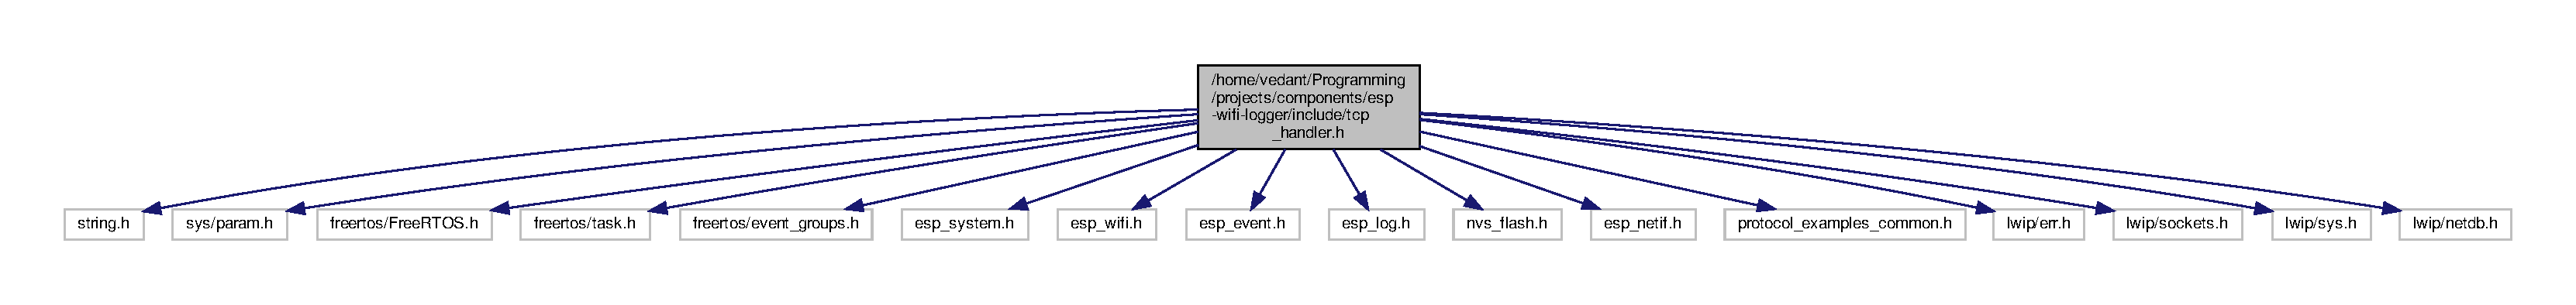
\includegraphics[width=350pt]{tcp__handler_8h__incl}
\end{center}
\end{figure}
This graph shows which files directly or indirectly include this file\+:\nopagebreak
\begin{figure}[H]
\begin{center}
\leavevmode
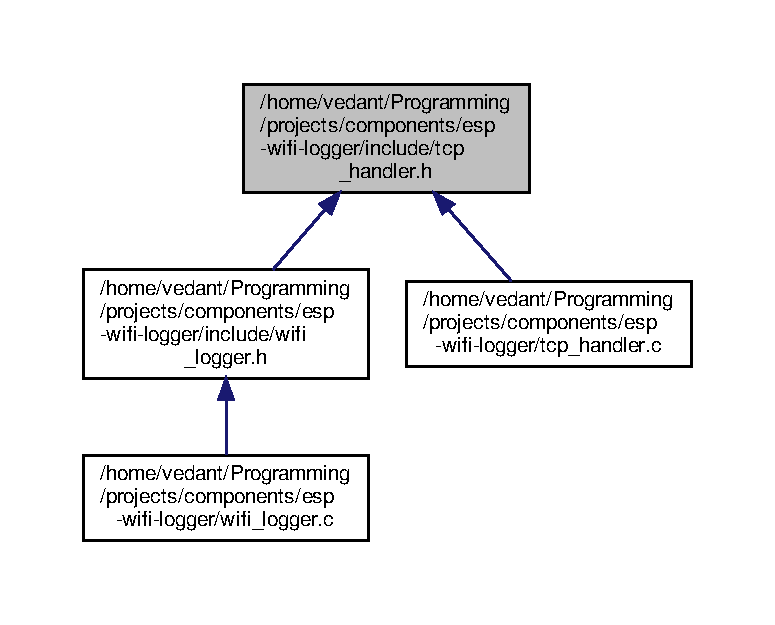
\includegraphics[width=350pt]{tcp__handler_8h__dep__incl}
\end{center}
\end{figure}
\subsection*{Classes}
\begin{DoxyCompactItemize}
\item 
struct \hyperlink{structtcp__network__data}{tcp\+\_\+network\+\_\+data}
\end{DoxyCompactItemize}
\subsection*{Macros}
\begin{DoxyCompactItemize}
\item 
\#define \hyperlink{tcp__handler_8h_a30e0c38ad4a5d0a16bfdd52ff64189b4}{T\+C\+P\+\_\+\+H\+O\+S\+T\+\_\+\+I\+P\+\_\+\+A\+D\+DR}~C\+O\+N\+F\+I\+G\+\_\+\+S\+E\+R\+V\+E\+R\+\_\+\+I\+P\+\_\+\+A\+D\+D\+R\+E\+SS
\item 
\#define \hyperlink{tcp__handler_8h_a637b73f06ee87043251d022f87a8f3d4}{T\+C\+P\+\_\+\+P\+O\+RT}~C\+O\+N\+F\+I\+G\+\_\+\+S\+E\+R\+V\+E\+R\+\_\+\+P\+O\+RT
\end{DoxyCompactItemize}
\subsection*{Functions}
\begin{DoxyCompactItemize}
\item 
void \hyperlink{tcp__handler_8h_a6be7633691ba5c012155871a84ade82e}{tcp\+\_\+network\+\_\+manager} (struct \hyperlink{structtcp__network__data}{tcp\+\_\+network\+\_\+data} $\ast$nm)
\begin{DoxyCompactList}\small\item\em Manages T\+CP connection to the server. \end{DoxyCompactList}\item 
int \hyperlink{tcp__handler_8h_a0ca62b309e39660b29ee7605b099ee54}{tcp\+\_\+send\+\_\+data} (struct \hyperlink{structtcp__network__data}{tcp\+\_\+network\+\_\+data} $\ast$nm, char $\ast$payload)
\begin{DoxyCompactList}\small\item\em Sends data to the server through a T\+CP socket. \end{DoxyCompactList}\item 
char $\ast$ \hyperlink{tcp__handler_8h_ae58555e8930155fcea5b1d16915db87b}{tcp\+\_\+recieve\+\_\+data} (struct \hyperlink{structtcp__network__data}{tcp\+\_\+network\+\_\+data} $\ast$nm)
\begin{DoxyCompactList}\small\item\em Receives data from T\+CP server. \end{DoxyCompactList}\item 
void \hyperlink{tcp__handler_8h_a6d6a248c21ebfece9f52fa7b580fabb5}{tcp\+\_\+close\+\_\+network\+\_\+manager} (struct \hyperlink{structtcp__network__data}{tcp\+\_\+network\+\_\+data} $\ast$nm)
\begin{DoxyCompactList}\small\item\em Shutdown active connection, deallocate memory. \end{DoxyCompactList}\end{DoxyCompactItemize}


\subsection{Macro Definition Documentation}
\mbox{\Hypertarget{tcp__handler_8h_a30e0c38ad4a5d0a16bfdd52ff64189b4}\label{tcp__handler_8h_a30e0c38ad4a5d0a16bfdd52ff64189b4}} 
\index{tcp\+\_\+handler.\+h@{tcp\+\_\+handler.\+h}!T\+C\+P\+\_\+\+H\+O\+S\+T\+\_\+\+I\+P\+\_\+\+A\+D\+DR@{T\+C\+P\+\_\+\+H\+O\+S\+T\+\_\+\+I\+P\+\_\+\+A\+D\+DR}}
\index{T\+C\+P\+\_\+\+H\+O\+S\+T\+\_\+\+I\+P\+\_\+\+A\+D\+DR@{T\+C\+P\+\_\+\+H\+O\+S\+T\+\_\+\+I\+P\+\_\+\+A\+D\+DR}!tcp\+\_\+handler.\+h@{tcp\+\_\+handler.\+h}}
\subsubsection{\texorpdfstring{T\+C\+P\+\_\+\+H\+O\+S\+T\+\_\+\+I\+P\+\_\+\+A\+D\+DR}{TCP\_HOST\_IP\_ADDR}}
{\footnotesize\ttfamily \#define T\+C\+P\+\_\+\+H\+O\+S\+T\+\_\+\+I\+P\+\_\+\+A\+D\+DR~C\+O\+N\+F\+I\+G\+\_\+\+S\+E\+R\+V\+E\+R\+\_\+\+I\+P\+\_\+\+A\+D\+D\+R\+E\+SS}

\mbox{\Hypertarget{tcp__handler_8h_a637b73f06ee87043251d022f87a8f3d4}\label{tcp__handler_8h_a637b73f06ee87043251d022f87a8f3d4}} 
\index{tcp\+\_\+handler.\+h@{tcp\+\_\+handler.\+h}!T\+C\+P\+\_\+\+P\+O\+RT@{T\+C\+P\+\_\+\+P\+O\+RT}}
\index{T\+C\+P\+\_\+\+P\+O\+RT@{T\+C\+P\+\_\+\+P\+O\+RT}!tcp\+\_\+handler.\+h@{tcp\+\_\+handler.\+h}}
\subsubsection{\texorpdfstring{T\+C\+P\+\_\+\+P\+O\+RT}{TCP\_PORT}}
{\footnotesize\ttfamily \#define T\+C\+P\+\_\+\+P\+O\+RT~C\+O\+N\+F\+I\+G\+\_\+\+S\+E\+R\+V\+E\+R\+\_\+\+P\+O\+RT}



\subsection{Function Documentation}
\mbox{\Hypertarget{tcp__handler_8h_a6d6a248c21ebfece9f52fa7b580fabb5}\label{tcp__handler_8h_a6d6a248c21ebfece9f52fa7b580fabb5}} 
\index{tcp\+\_\+handler.\+h@{tcp\+\_\+handler.\+h}!tcp\+\_\+close\+\_\+network\+\_\+manager@{tcp\+\_\+close\+\_\+network\+\_\+manager}}
\index{tcp\+\_\+close\+\_\+network\+\_\+manager@{tcp\+\_\+close\+\_\+network\+\_\+manager}!tcp\+\_\+handler.\+h@{tcp\+\_\+handler.\+h}}
\subsubsection{\texorpdfstring{tcp\+\_\+close\+\_\+network\+\_\+manager()}{tcp\_close\_network\_manager()}}
{\footnotesize\ttfamily void tcp\+\_\+close\+\_\+network\+\_\+manager (\begin{DoxyParamCaption}\item[{struct \hyperlink{structtcp__network__data}{tcp\+\_\+network\+\_\+data} $\ast$}]{nm }\end{DoxyParamCaption})}



Shutdown active connection, deallocate memory. 


\begin{DoxyParams}{Parameters}
{\em nm} & \hyperlink{structtcp__network__data}{tcp\+\_\+network\+\_\+data} struct which contains connection info \\
\hline
\end{DoxyParams}
\begin{DoxyReturn}{Returns}
void 
\end{DoxyReturn}
\mbox{\Hypertarget{tcp__handler_8h_a6be7633691ba5c012155871a84ade82e}\label{tcp__handler_8h_a6be7633691ba5c012155871a84ade82e}} 
\index{tcp\+\_\+handler.\+h@{tcp\+\_\+handler.\+h}!tcp\+\_\+network\+\_\+manager@{tcp\+\_\+network\+\_\+manager}}
\index{tcp\+\_\+network\+\_\+manager@{tcp\+\_\+network\+\_\+manager}!tcp\+\_\+handler.\+h@{tcp\+\_\+handler.\+h}}
\subsubsection{\texorpdfstring{tcp\+\_\+network\+\_\+manager()}{tcp\_network\_manager()}}
{\footnotesize\ttfamily void tcp\+\_\+network\+\_\+manager (\begin{DoxyParamCaption}\item[{struct \hyperlink{structtcp__network__data}{tcp\+\_\+network\+\_\+data} $\ast$}]{nm }\end{DoxyParamCaption})}



Manages T\+CP connection to the server. 


\begin{DoxyParams}{Parameters}
{\em nm} & \hyperlink{structtcp__network__data}{tcp\+\_\+network\+\_\+data} struct which contains necessary data for a T\+CP connection \\
\hline
\end{DoxyParams}
\begin{DoxyReturn}{Returns}
void 
\end{DoxyReturn}
\mbox{\Hypertarget{tcp__handler_8h_ae58555e8930155fcea5b1d16915db87b}\label{tcp__handler_8h_ae58555e8930155fcea5b1d16915db87b}} 
\index{tcp\+\_\+handler.\+h@{tcp\+\_\+handler.\+h}!tcp\+\_\+recieve\+\_\+data@{tcp\+\_\+recieve\+\_\+data}}
\index{tcp\+\_\+recieve\+\_\+data@{tcp\+\_\+recieve\+\_\+data}!tcp\+\_\+handler.\+h@{tcp\+\_\+handler.\+h}}
\subsubsection{\texorpdfstring{tcp\+\_\+recieve\+\_\+data()}{tcp\_recieve\_data()}}
{\footnotesize\ttfamily char$\ast$ tcp\+\_\+recieve\+\_\+data (\begin{DoxyParamCaption}\item[{struct \hyperlink{structtcp__network__data}{tcp\+\_\+network\+\_\+data} $\ast$}]{nm }\end{DoxyParamCaption})}



Receives data from T\+CP server. 


\begin{DoxyParams}{Parameters}
{\em nm} & \hyperlink{structtcp__network__data}{tcp\+\_\+network\+\_\+data} struct which contains connection info \\
\hline
\end{DoxyParams}
\begin{DoxyReturn}{Returns}
char array which contains data received 
\end{DoxyReturn}
\mbox{\Hypertarget{tcp__handler_8h_a0ca62b309e39660b29ee7605b099ee54}\label{tcp__handler_8h_a0ca62b309e39660b29ee7605b099ee54}} 
\index{tcp\+\_\+handler.\+h@{tcp\+\_\+handler.\+h}!tcp\+\_\+send\+\_\+data@{tcp\+\_\+send\+\_\+data}}
\index{tcp\+\_\+send\+\_\+data@{tcp\+\_\+send\+\_\+data}!tcp\+\_\+handler.\+h@{tcp\+\_\+handler.\+h}}
\subsubsection{\texorpdfstring{tcp\+\_\+send\+\_\+data()}{tcp\_send\_data()}}
{\footnotesize\ttfamily int tcp\+\_\+send\+\_\+data (\begin{DoxyParamCaption}\item[{struct \hyperlink{structtcp__network__data}{tcp\+\_\+network\+\_\+data} $\ast$}]{nm,  }\item[{char $\ast$}]{payload }\end{DoxyParamCaption})}



Sends data to the server through a T\+CP socket. 


\begin{DoxyParams}{Parameters}
{\em nm} & A pointer to \hyperlink{structtcp__network__data}{tcp\+\_\+network\+\_\+data} struct \\
\hline
{\em payload} & char array which contains data to be sent \\
\hline
\end{DoxyParams}
\begin{DoxyReturn}{Returns}
int -\/ returns -\/1 if sending failed, number of bytes sent if successfully sent the data 
\end{DoxyReturn}

\hypertarget{udp__handler_8h}{}\section{/home/vedant/\+Programming/projects/components/esp-\/wifi-\/logger/include/udp\+\_\+handler.h File Reference}
\label{udp__handler_8h}\index{/home/vedant/\+Programming/projects/components/esp-\/wifi-\/logger/include/udp\+\_\+handler.\+h@{/home/vedant/\+Programming/projects/components/esp-\/wifi-\/logger/include/udp\+\_\+handler.\+h}}
{\ttfamily \#include $<$string.\+h$>$}\newline
{\ttfamily \#include $<$sys/param.\+h$>$}\newline
{\ttfamily \#include \char`\"{}freertos/\+Free\+R\+T\+O\+S.\+h\char`\"{}}\newline
{\ttfamily \#include \char`\"{}freertos/task.\+h\char`\"{}}\newline
{\ttfamily \#include \char`\"{}freertos/event\+\_\+groups.\+h\char`\"{}}\newline
{\ttfamily \#include \char`\"{}esp\+\_\+system.\+h\char`\"{}}\newline
{\ttfamily \#include \char`\"{}esp\+\_\+wifi.\+h\char`\"{}}\newline
{\ttfamily \#include \char`\"{}esp\+\_\+event.\+h\char`\"{}}\newline
{\ttfamily \#include \char`\"{}esp\+\_\+log.\+h\char`\"{}}\newline
{\ttfamily \#include \char`\"{}nvs\+\_\+flash.\+h\char`\"{}}\newline
{\ttfamily \#include \char`\"{}esp\+\_\+netif.\+h\char`\"{}}\newline
{\ttfamily \#include \char`\"{}protocol\+\_\+examples\+\_\+common.\+h\char`\"{}}\newline
{\ttfamily \#include \char`\"{}lwip/err.\+h\char`\"{}}\newline
{\ttfamily \#include \char`\"{}lwip/sockets.\+h\char`\"{}}\newline
{\ttfamily \#include \char`\"{}lwip/sys.\+h\char`\"{}}\newline
{\ttfamily \#include $<$lwip/netdb.\+h$>$}\newline
Include dependency graph for udp\+\_\+handler.\+h\+:
\nopagebreak
\begin{figure}[H]
\begin{center}
\leavevmode
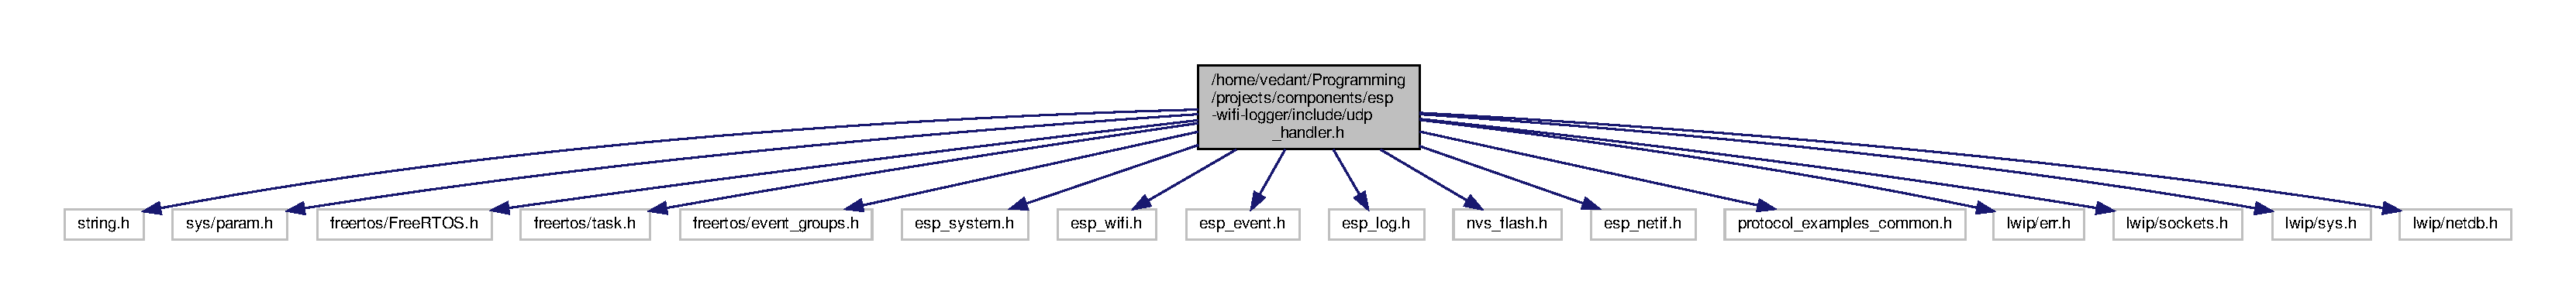
\includegraphics[width=350pt]{udp__handler_8h__incl}
\end{center}
\end{figure}
This graph shows which files directly or indirectly include this file\+:
\nopagebreak
\begin{figure}[H]
\begin{center}
\leavevmode
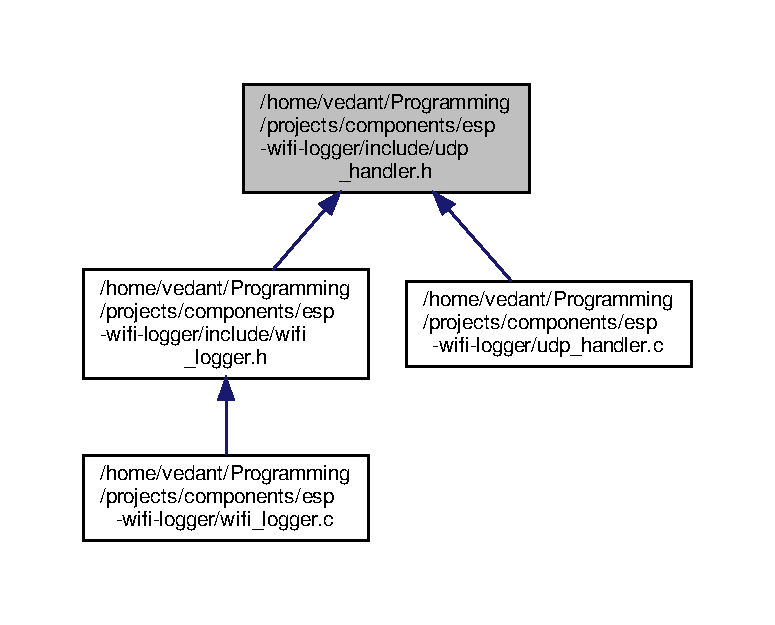
\includegraphics[width=350pt]{udp__handler_8h__dep__incl}
\end{center}
\end{figure}
\subsection*{Classes}
\begin{DoxyCompactItemize}
\item 
struct \hyperlink{structnetwork__data}{network\+\_\+data}
\end{DoxyCompactItemize}
\subsection*{Macros}
\begin{DoxyCompactItemize}
\item 
\#define \hyperlink{udp__handler_8h_a0755be366390c472fea523dda78961d3}{H\+O\+S\+T\+\_\+\+I\+P\+\_\+\+A\+D\+DR}~C\+O\+N\+F\+I\+G\+\_\+\+S\+E\+R\+V\+E\+R\+\_\+\+I\+P\+\_\+\+A\+D\+D\+R\+E\+SS
\item 
\#define \hyperlink{udp__handler_8h_a614217d263be1fb1a5f76e2ff7be19a2}{P\+O\+RT}~C\+O\+N\+F\+I\+G\+\_\+\+S\+E\+R\+V\+E\+R\+\_\+\+P\+O\+RT
\end{DoxyCompactItemize}
\subsection*{Functions}
\begin{DoxyCompactItemize}
\item 
void \hyperlink{udp__handler_8h_a412aa3402fc47e327861b48a04c3c08a}{network\+\_\+manager} (struct \hyperlink{structnetwork__data}{network\+\_\+data} $\ast$nm)
\begin{DoxyCompactList}\small\item\em Manages U\+DP connection to the server. \end{DoxyCompactList}\item 
int \hyperlink{udp__handler_8h_a7ddbd791c1d13c96db95eba36aae6145}{send\+\_\+data} (struct \hyperlink{structnetwork__data}{network\+\_\+data} $\ast$nm, char $\ast$payload)
\begin{DoxyCompactList}\small\item\em Sends data to the server through a U\+DP socket. \end{DoxyCompactList}\item 
char $\ast$ \hyperlink{udp__handler_8h_afe419fdd19f7194dcf9c9e6d00118224}{recieve\+\_\+data} (struct \hyperlink{structnetwork__data}{network\+\_\+data} $\ast$nm)
\begin{DoxyCompactList}\small\item\em Receives data from U\+DP server. \end{DoxyCompactList}\item 
void \hyperlink{udp__handler_8h_a3e138ed94c89bd74c249c9f4a1a4c642}{close\+\_\+network\+\_\+manager} (struct \hyperlink{structnetwork__data}{network\+\_\+data} $\ast$nm)
\begin{DoxyCompactList}\small\item\em Shutdown active connection, deallocate memory. \end{DoxyCompactList}\end{DoxyCompactItemize}


\subsection{Macro Definition Documentation}
\mbox{\Hypertarget{udp__handler_8h_a0755be366390c472fea523dda78961d3}\label{udp__handler_8h_a0755be366390c472fea523dda78961d3}} 
\index{udp\+\_\+handler.\+h@{udp\+\_\+handler.\+h}!H\+O\+S\+T\+\_\+\+I\+P\+\_\+\+A\+D\+DR@{H\+O\+S\+T\+\_\+\+I\+P\+\_\+\+A\+D\+DR}}
\index{H\+O\+S\+T\+\_\+\+I\+P\+\_\+\+A\+D\+DR@{H\+O\+S\+T\+\_\+\+I\+P\+\_\+\+A\+D\+DR}!udp\+\_\+handler.\+h@{udp\+\_\+handler.\+h}}
\subsubsection{\texorpdfstring{H\+O\+S\+T\+\_\+\+I\+P\+\_\+\+A\+D\+DR}{HOST\_IP\_ADDR}}
{\footnotesize\ttfamily \#define H\+O\+S\+T\+\_\+\+I\+P\+\_\+\+A\+D\+DR~C\+O\+N\+F\+I\+G\+\_\+\+S\+E\+R\+V\+E\+R\+\_\+\+I\+P\+\_\+\+A\+D\+D\+R\+E\+SS}

\mbox{\Hypertarget{udp__handler_8h_a614217d263be1fb1a5f76e2ff7be19a2}\label{udp__handler_8h_a614217d263be1fb1a5f76e2ff7be19a2}} 
\index{udp\+\_\+handler.\+h@{udp\+\_\+handler.\+h}!P\+O\+RT@{P\+O\+RT}}
\index{P\+O\+RT@{P\+O\+RT}!udp\+\_\+handler.\+h@{udp\+\_\+handler.\+h}}
\subsubsection{\texorpdfstring{P\+O\+RT}{PORT}}
{\footnotesize\ttfamily \#define P\+O\+RT~C\+O\+N\+F\+I\+G\+\_\+\+S\+E\+R\+V\+E\+R\+\_\+\+P\+O\+RT}



\subsection{Function Documentation}
\mbox{\Hypertarget{udp__handler_8h_a3e138ed94c89bd74c249c9f4a1a4c642}\label{udp__handler_8h_a3e138ed94c89bd74c249c9f4a1a4c642}} 
\index{udp\+\_\+handler.\+h@{udp\+\_\+handler.\+h}!close\+\_\+network\+\_\+manager@{close\+\_\+network\+\_\+manager}}
\index{close\+\_\+network\+\_\+manager@{close\+\_\+network\+\_\+manager}!udp\+\_\+handler.\+h@{udp\+\_\+handler.\+h}}
\subsubsection{\texorpdfstring{close\+\_\+network\+\_\+manager()}{close\_network\_manager()}}
{\footnotesize\ttfamily void close\+\_\+network\+\_\+manager (\begin{DoxyParamCaption}\item[{struct \hyperlink{structnetwork__data}{network\+\_\+data} $\ast$}]{nm }\end{DoxyParamCaption})}



Shutdown active connection, deallocate memory. 


\begin{DoxyParams}{Parameters}
{\em nm} & \hyperlink{structtcp__network__data}{tcp\+\_\+network\+\_\+data} struct which contains connection info \\
\hline
\end{DoxyParams}
\begin{DoxyReturn}{Returns}
void 
\end{DoxyReturn}
\mbox{\Hypertarget{udp__handler_8h_a412aa3402fc47e327861b48a04c3c08a}\label{udp__handler_8h_a412aa3402fc47e327861b48a04c3c08a}} 
\index{udp\+\_\+handler.\+h@{udp\+\_\+handler.\+h}!network\+\_\+manager@{network\+\_\+manager}}
\index{network\+\_\+manager@{network\+\_\+manager}!udp\+\_\+handler.\+h@{udp\+\_\+handler.\+h}}
\subsubsection{\texorpdfstring{network\+\_\+manager()}{network\_manager()}}
{\footnotesize\ttfamily void network\+\_\+manager (\begin{DoxyParamCaption}\item[{struct \hyperlink{structnetwork__data}{network\+\_\+data} $\ast$}]{nm }\end{DoxyParamCaption})}



Manages U\+DP connection to the server. 


\begin{DoxyParams}{Parameters}
{\em nm} & \hyperlink{structnetwork__data}{network\+\_\+data} struct which contains necessary data for a U\+DP connection \\
\hline
\end{DoxyParams}
\begin{DoxyReturn}{Returns}
void 
\end{DoxyReturn}
\mbox{\Hypertarget{udp__handler_8h_afe419fdd19f7194dcf9c9e6d00118224}\label{udp__handler_8h_afe419fdd19f7194dcf9c9e6d00118224}} 
\index{udp\+\_\+handler.\+h@{udp\+\_\+handler.\+h}!recieve\+\_\+data@{recieve\+\_\+data}}
\index{recieve\+\_\+data@{recieve\+\_\+data}!udp\+\_\+handler.\+h@{udp\+\_\+handler.\+h}}
\subsubsection{\texorpdfstring{recieve\+\_\+data()}{recieve\_data()}}
{\footnotesize\ttfamily char$\ast$ recieve\+\_\+data (\begin{DoxyParamCaption}\item[{struct \hyperlink{structnetwork__data}{network\+\_\+data} $\ast$}]{nm }\end{DoxyParamCaption})}



Receives data from U\+DP server. 


\begin{DoxyParams}{Parameters}
{\em nm} & \hyperlink{structnetwork__data}{network\+\_\+data} struct which contains connection info \\
\hline
\end{DoxyParams}
\begin{DoxyReturn}{Returns}
char array which contains data received 
\end{DoxyReturn}
\mbox{\Hypertarget{udp__handler_8h_a7ddbd791c1d13c96db95eba36aae6145}\label{udp__handler_8h_a7ddbd791c1d13c96db95eba36aae6145}} 
\index{udp\+\_\+handler.\+h@{udp\+\_\+handler.\+h}!send\+\_\+data@{send\+\_\+data}}
\index{send\+\_\+data@{send\+\_\+data}!udp\+\_\+handler.\+h@{udp\+\_\+handler.\+h}}
\subsubsection{\texorpdfstring{send\+\_\+data()}{send\_data()}}
{\footnotesize\ttfamily int send\+\_\+data (\begin{DoxyParamCaption}\item[{struct \hyperlink{structnetwork__data}{network\+\_\+data} $\ast$}]{nm,  }\item[{char $\ast$}]{payload }\end{DoxyParamCaption})}



Sends data to the server through a U\+DP socket. 


\begin{DoxyParams}{Parameters}
{\em nm} & A pointer to \hyperlink{structnetwork__data}{network\+\_\+data} struct \\
\hline
{\em payload} & char array which contains data to be sent \\
\hline
\end{DoxyParams}
\begin{DoxyReturn}{Returns}
int -\/ returns -\/1 if sending failed, number of bytes sent if successfully sent the data 
\end{DoxyReturn}

\hypertarget{utils_8h}{}\section{/home/vedant/\+Programming/projects/components/esp-\/wifi-\/logger/include/utils.h File Reference}
\label{utils_8h}\index{/home/vedant/\+Programming/projects/components/esp-\/wifi-\/logger/include/utils.\+h@{/home/vedant/\+Programming/projects/components/esp-\/wifi-\/logger/include/utils.\+h}}
This graph shows which files directly or indirectly include this file\+:
\nopagebreak
\begin{figure}[H]
\begin{center}
\leavevmode
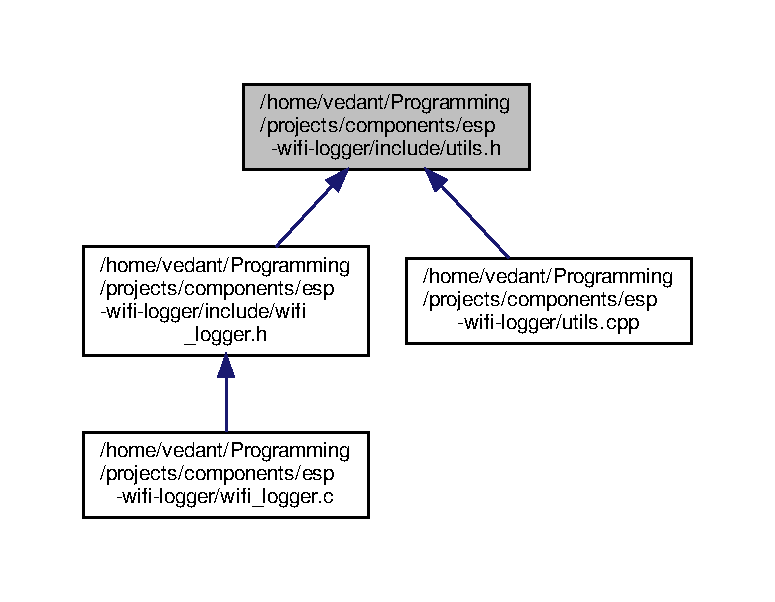
\includegraphics[width=350pt]{utils_8h__dep__incl}
\end{center}
\end{figure}
\subsection*{Functions}
\begin{DoxyCompactItemize}
\item 
char $\ast$ \hyperlink{utils_8h_af768902cbc75dc282b88515dd045b7b5}{generate\+\_\+log\+\_\+message\+\_\+timestamp} (uint32\+\_\+t timestamp, char $\ast$log\+\_\+message)
\end{DoxyCompactItemize}


\subsection{Function Documentation}
\mbox{\Hypertarget{utils_8h_af768902cbc75dc282b88515dd045b7b5}\label{utils_8h_af768902cbc75dc282b88515dd045b7b5}} 
\index{utils.\+h@{utils.\+h}!generate\+\_\+log\+\_\+message\+\_\+timestamp@{generate\+\_\+log\+\_\+message\+\_\+timestamp}}
\index{generate\+\_\+log\+\_\+message\+\_\+timestamp@{generate\+\_\+log\+\_\+message\+\_\+timestamp}!utils.\+h@{utils.\+h}}
\subsubsection{\texorpdfstring{generate\+\_\+log\+\_\+message\+\_\+timestamp()}{generate\_log\_message\_timestamp()}}
{\footnotesize\ttfamily char$\ast$ generate\+\_\+log\+\_\+message\+\_\+timestamp (\begin{DoxyParamCaption}\item[{uint32\+\_\+t}]{timestamp,  }\item[{char $\ast$}]{log\+\_\+message }\end{DoxyParamCaption})}


\hypertarget{wifi__logger_8h}{}\section{/home/vedant/\+Programming/projects/components/esp-\/wifi-\/logger/include/wifi\+\_\+logger.h File Reference}
\label{wifi__logger_8h}\index{/home/vedant/\+Programming/projects/components/esp-\/wifi-\/logger/include/wifi\+\_\+logger.\+h@{/home/vedant/\+Programming/projects/components/esp-\/wifi-\/logger/include/wifi\+\_\+logger.\+h}}
{\ttfamily \#include \char`\"{}tcp\+\_\+handler.\+h\char`\"{}}\newline
{\ttfamily \#include \char`\"{}udp\+\_\+handler.\+h\char`\"{}}\newline
{\ttfamily \#include \char`\"{}utils.\+h\char`\"{}}\newline
{\ttfamily \#include \char`\"{}freertos/\+Free\+R\+T\+O\+S.\+h\char`\"{}}\newline
{\ttfamily \#include \char`\"{}freertos/task.\+h\char`\"{}}\newline
{\ttfamily \#include \char`\"{}esp\+\_\+system.\+h\char`\"{}}\newline
{\ttfamily \#include \char`\"{}freertos/queue.\+h\char`\"{}}\newline
{\ttfamily \#include $<$stdlib.\+h$>$}\newline
{\ttfamily \#include $<$string.\+h$>$}\newline
Include dependency graph for wifi\+\_\+logger.\+h\+:\nopagebreak
\begin{figure}[H]
\begin{center}
\leavevmode
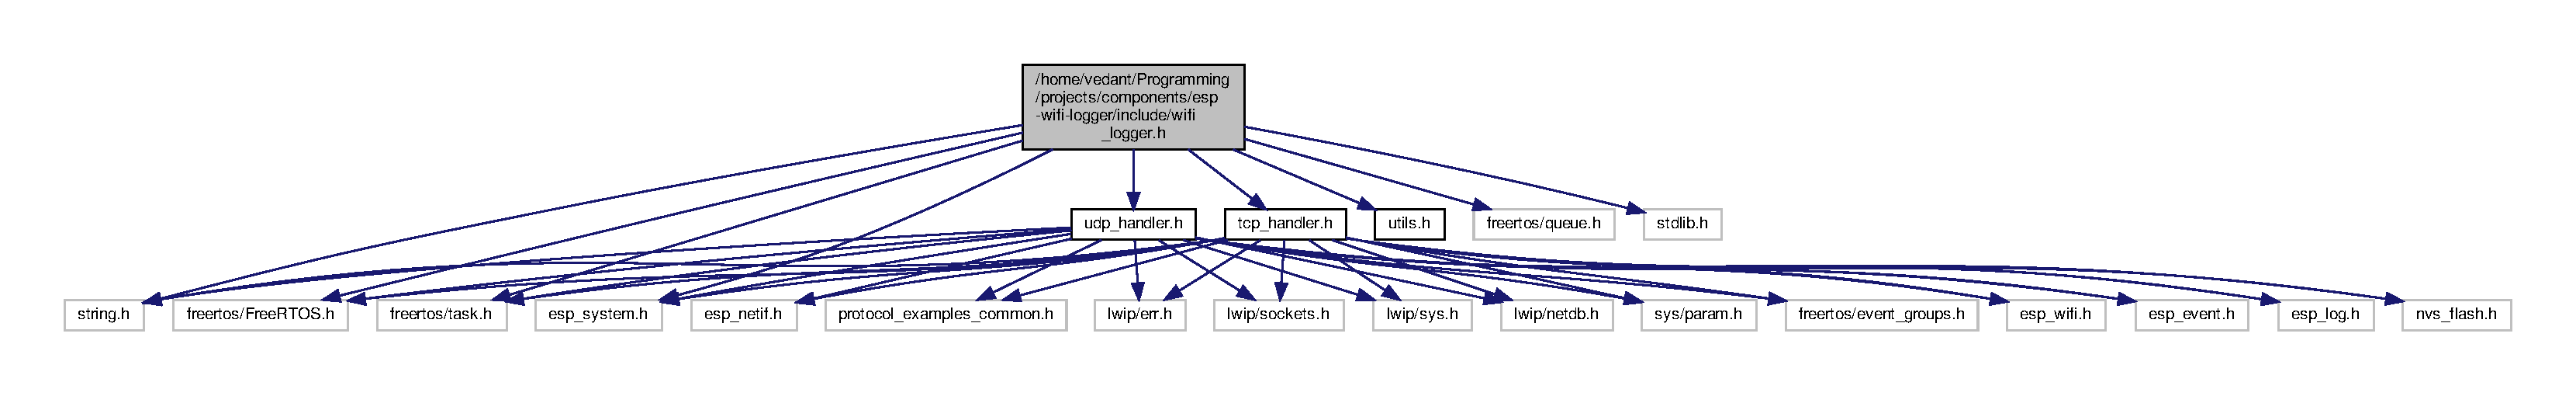
\includegraphics[width=350pt]{wifi__logger_8h__incl}
\end{center}
\end{figure}
This graph shows which files directly or indirectly include this file\+:\nopagebreak
\begin{figure}[H]
\begin{center}
\leavevmode
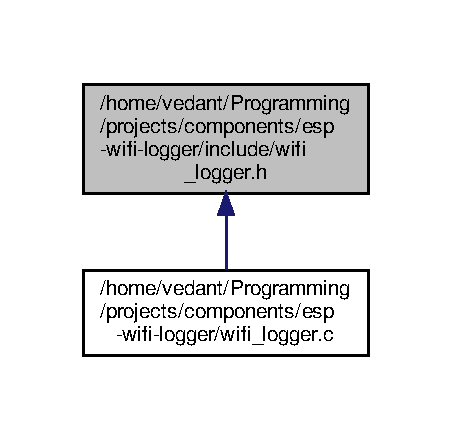
\includegraphics[width=217pt]{wifi__logger_8h__dep__incl}
\end{center}
\end{figure}
\subsection*{Macros}
\begin{DoxyCompactItemize}
\item 
\#define \hyperlink{wifi__logger_8h_a81a6fc89c7bc286cb7360b155b1901bf}{M\+E\+S\+S\+A\+G\+E\+\_\+\+Q\+U\+E\+U\+E\+\_\+\+S\+I\+ZE}~C\+O\+N\+F\+I\+G\+\_\+\+M\+E\+S\+S\+A\+G\+E\+\_\+\+Q\+U\+E\+U\+E\+\_\+\+S\+I\+ZE
\item 
\#define \hyperlink{wifi__logger_8h_a6b20d41d6252e9871430c242cb1a56e7}{B\+U\+F\+F\+E\+R\+\_\+\+S\+I\+ZE}~C\+O\+N\+F\+I\+G\+\_\+\+B\+U\+F\+F\+E\+R\+\_\+\+S\+I\+ZE
\item 
\#define \hyperlink{wifi__logger_8h_a6423a880df59733d2d9b509c7718d3a9}{S\+T\+A\+C\+K\+\_\+\+S\+I\+ZE}~C\+O\+N\+F\+I\+G\+\_\+\+M\+E\+S\+S\+A\+G\+E\+\_\+\+Q\+U\+E\+U\+E\+\_\+\+S\+I\+ZE$\ast$8
\item 
\#define \hyperlink{wifi__logger_8h_a2e13ac2e5cc7918fe456d748c7db19ef}{wifi\+\_\+log}(T\+AG,  fmt, ...)~\hyperlink{wifi__logger_8c_a479c62eb886c1c0aa898a033916bb653}{generate\+\_\+log\+\_\+message}(T\+AG, \+\_\+\+\_\+\+L\+I\+N\+E\+\_\+\+\_\+, \+\_\+\+\_\+func\+\_\+\+\_\+, fmt, \+\_\+\+\_\+\+V\+A\+\_\+\+A\+R\+G\+S\+\_\+\+\_\+);
\end{DoxyCompactItemize}
\subsection*{Functions}
\begin{DoxyCompactItemize}
\item 
esp\+\_\+err\+\_\+t \hyperlink{wifi__logger_8h_a320afeaba56579760e7e3185a3d1fa02}{init\+\_\+queue} (void)
\begin{DoxyCompactList}\small\item\em Initialises message queue. \end{DoxyCompactList}\item 
void \hyperlink{wifi__logger_8h_aea5e8c4231b83bde5f8f0f4556271aba}{init\+\_\+wifi} (void)
\begin{DoxyCompactList}\small\item\em Initialises and connects to wifi. \end{DoxyCompactList}\item 
esp\+\_\+err\+\_\+t \hyperlink{wifi__logger_8h_a2261c877b2e047a36b7df77259b689ec}{send\+\_\+to\+\_\+queue} (const char $\ast$log\+\_\+message)
\begin{DoxyCompactList}\small\item\em Sends log message to message queue. \end{DoxyCompactList}\item 
char $\ast$ \hyperlink{wifi__logger_8h_ad28af408449f666a77441f0120a6a228}{receive\+\_\+from\+\_\+queue} (void)
\begin{DoxyCompactList}\small\item\em Receive data from queue. \end{DoxyCompactList}\item 
void \hyperlink{wifi__logger_8h_a479c62eb886c1c0aa898a033916bb653}{generate\+\_\+log\+\_\+message} (const char $\ast$T\+AG, int line, const char $\ast$func, const char $\ast$fmt,...)
\begin{DoxyCompactList}\small\item\em generates log message, of the format generated by E\+S\+P\+\_\+\+L\+OG function \end{DoxyCompactList}\item 
void \hyperlink{wifi__logger_8h_a8e612786031d82bb0eac8affe469ed2c}{start\+\_\+wifi\+\_\+logger} (void)
\begin{DoxyCompactList}\small\item\em wrapper function to start wifi logger \end{DoxyCompactList}\end{DoxyCompactItemize}
\subsection*{Variables}
\begin{DoxyCompactItemize}
\item 
Queue\+Handle\+\_\+t \hyperlink{wifi__logger_8h_afde8dfae74b6444a5a97ef478d33eb6e}{wifi\+\_\+logger\+\_\+queue}
\end{DoxyCompactItemize}


\subsection{Macro Definition Documentation}
\mbox{\Hypertarget{wifi__logger_8h_a6b20d41d6252e9871430c242cb1a56e7}\label{wifi__logger_8h_a6b20d41d6252e9871430c242cb1a56e7}} 
\index{wifi\+\_\+logger.\+h@{wifi\+\_\+logger.\+h}!B\+U\+F\+F\+E\+R\+\_\+\+S\+I\+ZE@{B\+U\+F\+F\+E\+R\+\_\+\+S\+I\+ZE}}
\index{B\+U\+F\+F\+E\+R\+\_\+\+S\+I\+ZE@{B\+U\+F\+F\+E\+R\+\_\+\+S\+I\+ZE}!wifi\+\_\+logger.\+h@{wifi\+\_\+logger.\+h}}
\subsubsection{\texorpdfstring{B\+U\+F\+F\+E\+R\+\_\+\+S\+I\+ZE}{BUFFER\_SIZE}}
{\footnotesize\ttfamily \#define B\+U\+F\+F\+E\+R\+\_\+\+S\+I\+ZE~C\+O\+N\+F\+I\+G\+\_\+\+B\+U\+F\+F\+E\+R\+\_\+\+S\+I\+ZE}

\mbox{\Hypertarget{wifi__logger_8h_a81a6fc89c7bc286cb7360b155b1901bf}\label{wifi__logger_8h_a81a6fc89c7bc286cb7360b155b1901bf}} 
\index{wifi\+\_\+logger.\+h@{wifi\+\_\+logger.\+h}!M\+E\+S\+S\+A\+G\+E\+\_\+\+Q\+U\+E\+U\+E\+\_\+\+S\+I\+ZE@{M\+E\+S\+S\+A\+G\+E\+\_\+\+Q\+U\+E\+U\+E\+\_\+\+S\+I\+ZE}}
\index{M\+E\+S\+S\+A\+G\+E\+\_\+\+Q\+U\+E\+U\+E\+\_\+\+S\+I\+ZE@{M\+E\+S\+S\+A\+G\+E\+\_\+\+Q\+U\+E\+U\+E\+\_\+\+S\+I\+ZE}!wifi\+\_\+logger.\+h@{wifi\+\_\+logger.\+h}}
\subsubsection{\texorpdfstring{M\+E\+S\+S\+A\+G\+E\+\_\+\+Q\+U\+E\+U\+E\+\_\+\+S\+I\+ZE}{MESSAGE\_QUEUE\_SIZE}}
{\footnotesize\ttfamily \#define M\+E\+S\+S\+A\+G\+E\+\_\+\+Q\+U\+E\+U\+E\+\_\+\+S\+I\+ZE~C\+O\+N\+F\+I\+G\+\_\+\+M\+E\+S\+S\+A\+G\+E\+\_\+\+Q\+U\+E\+U\+E\+\_\+\+S\+I\+ZE}

\mbox{\Hypertarget{wifi__logger_8h_a6423a880df59733d2d9b509c7718d3a9}\label{wifi__logger_8h_a6423a880df59733d2d9b509c7718d3a9}} 
\index{wifi\+\_\+logger.\+h@{wifi\+\_\+logger.\+h}!S\+T\+A\+C\+K\+\_\+\+S\+I\+ZE@{S\+T\+A\+C\+K\+\_\+\+S\+I\+ZE}}
\index{S\+T\+A\+C\+K\+\_\+\+S\+I\+ZE@{S\+T\+A\+C\+K\+\_\+\+S\+I\+ZE}!wifi\+\_\+logger.\+h@{wifi\+\_\+logger.\+h}}
\subsubsection{\texorpdfstring{S\+T\+A\+C\+K\+\_\+\+S\+I\+ZE}{STACK\_SIZE}}
{\footnotesize\ttfamily \#define S\+T\+A\+C\+K\+\_\+\+S\+I\+ZE~C\+O\+N\+F\+I\+G\+\_\+\+M\+E\+S\+S\+A\+G\+E\+\_\+\+Q\+U\+E\+U\+E\+\_\+\+S\+I\+ZE$\ast$8}

\mbox{\Hypertarget{wifi__logger_8h_a2e13ac2e5cc7918fe456d748c7db19ef}\label{wifi__logger_8h_a2e13ac2e5cc7918fe456d748c7db19ef}} 
\index{wifi\+\_\+logger.\+h@{wifi\+\_\+logger.\+h}!wifi\+\_\+log@{wifi\+\_\+log}}
\index{wifi\+\_\+log@{wifi\+\_\+log}!wifi\+\_\+logger.\+h@{wifi\+\_\+logger.\+h}}
\subsubsection{\texorpdfstring{wifi\+\_\+log}{wifi\_log}}
{\footnotesize\ttfamily \#define wifi\+\_\+log(\begin{DoxyParamCaption}\item[{}]{T\+AG,  }\item[{}]{fmt,  }\item[{}]{... }\end{DoxyParamCaption})~\hyperlink{wifi__logger_8c_a479c62eb886c1c0aa898a033916bb653}{generate\+\_\+log\+\_\+message}(T\+AG, \+\_\+\+\_\+\+L\+I\+N\+E\+\_\+\+\_\+, \+\_\+\+\_\+func\+\_\+\+\_\+, fmt, \+\_\+\+\_\+\+V\+A\+\_\+\+A\+R\+G\+S\+\_\+\+\_\+);}



\subsection{Function Documentation}
\mbox{\Hypertarget{wifi__logger_8h_a479c62eb886c1c0aa898a033916bb653}\label{wifi__logger_8h_a479c62eb886c1c0aa898a033916bb653}} 
\index{wifi\+\_\+logger.\+h@{wifi\+\_\+logger.\+h}!generate\+\_\+log\+\_\+message@{generate\+\_\+log\+\_\+message}}
\index{generate\+\_\+log\+\_\+message@{generate\+\_\+log\+\_\+message}!wifi\+\_\+logger.\+h@{wifi\+\_\+logger.\+h}}
\subsubsection{\texorpdfstring{generate\+\_\+log\+\_\+message()}{generate\_log\_message()}}
{\footnotesize\ttfamily void generate\+\_\+log\+\_\+message (\begin{DoxyParamCaption}\item[{const char $\ast$}]{T\+AG,  }\item[{int}]{line,  }\item[{const char $\ast$}]{func,  }\item[{const char $\ast$}]{fmt,  }\item[{}]{... }\end{DoxyParamCaption})}



generates log message, of the format generated by E\+S\+P\+\_\+\+L\+OG function 


\begin{DoxyParams}{Parameters}
{\em T\+AG} & Tag for the log message \\
\hline
{\em line} & line \\
\hline
{\em func} & func \\
\hline
{\em fmt} & fmt \\
\hline
\end{DoxyParams}
\mbox{\Hypertarget{wifi__logger_8h_a320afeaba56579760e7e3185a3d1fa02}\label{wifi__logger_8h_a320afeaba56579760e7e3185a3d1fa02}} 
\index{wifi\+\_\+logger.\+h@{wifi\+\_\+logger.\+h}!init\+\_\+queue@{init\+\_\+queue}}
\index{init\+\_\+queue@{init\+\_\+queue}!wifi\+\_\+logger.\+h@{wifi\+\_\+logger.\+h}}
\subsubsection{\texorpdfstring{init\+\_\+queue()}{init\_queue()}}
{\footnotesize\ttfamily esp\+\_\+err\+\_\+t init\+\_\+queue (\begin{DoxyParamCaption}\item[{void}]{ }\end{DoxyParamCaption})}



Initialises message queue. 

\begin{DoxyReturn}{Returns}
esp\+\_\+err\+\_\+t E\+S\+P\+\_\+\+OK -\/ if queue init sucessfully, E\+S\+P\+\_\+\+F\+A\+IL -\/ if queue init failed 
\end{DoxyReturn}
\mbox{\Hypertarget{wifi__logger_8h_aea5e8c4231b83bde5f8f0f4556271aba}\label{wifi__logger_8h_aea5e8c4231b83bde5f8f0f4556271aba}} 
\index{wifi\+\_\+logger.\+h@{wifi\+\_\+logger.\+h}!init\+\_\+wifi@{init\+\_\+wifi}}
\index{init\+\_\+wifi@{init\+\_\+wifi}!wifi\+\_\+logger.\+h@{wifi\+\_\+logger.\+h}}
\subsubsection{\texorpdfstring{init\+\_\+wifi()}{init\_wifi()}}
{\footnotesize\ttfamily void init\+\_\+wifi (\begin{DoxyParamCaption}\item[{void}]{ }\end{DoxyParamCaption})}



Initialises and connects to wifi. 

\mbox{\Hypertarget{wifi__logger_8h_ad28af408449f666a77441f0120a6a228}\label{wifi__logger_8h_ad28af408449f666a77441f0120a6a228}} 
\index{wifi\+\_\+logger.\+h@{wifi\+\_\+logger.\+h}!receive\+\_\+from\+\_\+queue@{receive\+\_\+from\+\_\+queue}}
\index{receive\+\_\+from\+\_\+queue@{receive\+\_\+from\+\_\+queue}!wifi\+\_\+logger.\+h@{wifi\+\_\+logger.\+h}}
\subsubsection{\texorpdfstring{receive\+\_\+from\+\_\+queue()}{receive\_from\_queue()}}
{\footnotesize\ttfamily char$\ast$ receive\+\_\+from\+\_\+queue (\begin{DoxyParamCaption}\item[{void}]{ }\end{DoxyParamCaption})}



Receive data from queue. 

\begin{DoxyReturn}{Returns}
char$\ast$ -\/ returns log message received from the queue, returns N\+U\+LL if error or timeout 
\end{DoxyReturn}
\mbox{\Hypertarget{wifi__logger_8h_a2261c877b2e047a36b7df77259b689ec}\label{wifi__logger_8h_a2261c877b2e047a36b7df77259b689ec}} 
\index{wifi\+\_\+logger.\+h@{wifi\+\_\+logger.\+h}!send\+\_\+to\+\_\+queue@{send\+\_\+to\+\_\+queue}}
\index{send\+\_\+to\+\_\+queue@{send\+\_\+to\+\_\+queue}!wifi\+\_\+logger.\+h@{wifi\+\_\+logger.\+h}}
\subsubsection{\texorpdfstring{send\+\_\+to\+\_\+queue()}{send\_to\_queue()}}
{\footnotesize\ttfamily esp\+\_\+err\+\_\+t send\+\_\+to\+\_\+queue (\begin{DoxyParamCaption}\item[{const char $\ast$}]{log\+\_\+message }\end{DoxyParamCaption})}



Sends log message to message queue. 


\begin{DoxyParams}{Parameters}
{\em log\+\_\+message} & log message to be sent to the queue \\
\hline
\end{DoxyParams}
\begin{DoxyReturn}{Returns}
esp\+\_\+err\+\_\+t E\+S\+P\+\_\+\+OK -\/ if queue init sucessfully, E\+S\+P\+\_\+\+F\+A\+IL -\/ if queue init failed 
\end{DoxyReturn}
\mbox{\Hypertarget{wifi__logger_8h_a8e612786031d82bb0eac8affe469ed2c}\label{wifi__logger_8h_a8e612786031d82bb0eac8affe469ed2c}} 
\index{wifi\+\_\+logger.\+h@{wifi\+\_\+logger.\+h}!start\+\_\+wifi\+\_\+logger@{start\+\_\+wifi\+\_\+logger}}
\index{start\+\_\+wifi\+\_\+logger@{start\+\_\+wifi\+\_\+logger}!wifi\+\_\+logger.\+h@{wifi\+\_\+logger.\+h}}
\subsubsection{\texorpdfstring{start\+\_\+wifi\+\_\+logger()}{start\_wifi\_logger()}}
{\footnotesize\ttfamily void start\+\_\+wifi\+\_\+logger (\begin{DoxyParamCaption}\item[{void}]{ }\end{DoxyParamCaption})}



wrapper function to start wifi logger 



\subsection{Variable Documentation}
\mbox{\Hypertarget{wifi__logger_8h_afde8dfae74b6444a5a97ef478d33eb6e}\label{wifi__logger_8h_afde8dfae74b6444a5a97ef478d33eb6e}} 
\index{wifi\+\_\+logger.\+h@{wifi\+\_\+logger.\+h}!wifi\+\_\+logger\+\_\+queue@{wifi\+\_\+logger\+\_\+queue}}
\index{wifi\+\_\+logger\+\_\+queue@{wifi\+\_\+logger\+\_\+queue}!wifi\+\_\+logger.\+h@{wifi\+\_\+logger.\+h}}
\subsubsection{\texorpdfstring{wifi\+\_\+logger\+\_\+queue}{wifi\_logger\_queue}}
{\footnotesize\ttfamily Queue\+Handle\+\_\+t wifi\+\_\+logger\+\_\+queue}


\hypertarget{_r_e_a_d_m_e_8md}{}\section{/home/vedant/\+Programming/projects/components/esp-\/wifi-\/logger/\+R\+E\+A\+D\+ME.md File Reference}
\label{_r_e_a_d_m_e_8md}\index{/home/vedant/\+Programming/projects/components/esp-\/wifi-\/logger/\+R\+E\+A\+D\+M\+E.\+md@{/home/vedant/\+Programming/projects/components/esp-\/wifi-\/logger/\+R\+E\+A\+D\+M\+E.\+md}}

\hypertarget{tcp__handler_8c}{}\section{/home/vedant/\+Programming/projects/components/esp-\/wifi-\/logger/tcp\+\_\+handler.c File Reference}
\label{tcp__handler_8c}\index{/home/vedant/\+Programming/projects/components/esp-\/wifi-\/logger/tcp\+\_\+handler.\+c@{/home/vedant/\+Programming/projects/components/esp-\/wifi-\/logger/tcp\+\_\+handler.\+c}}
{\ttfamily \#include \char`\"{}tcp\+\_\+handler.\+h\char`\"{}}\newline
Include dependency graph for tcp\+\_\+handler.\+c\+:
\nopagebreak
\begin{figure}[H]
\begin{center}
\leavevmode
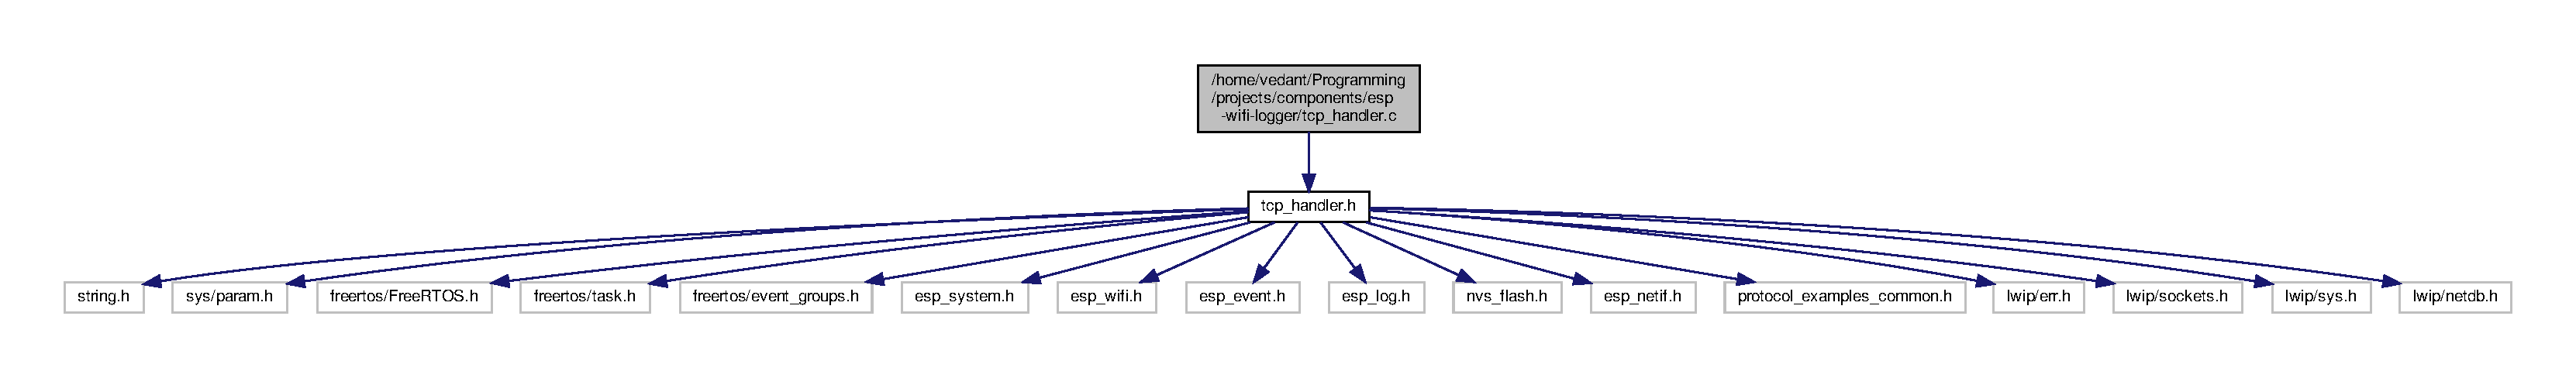
\includegraphics[width=350pt]{tcp__handler_8c__incl}
\end{center}
\end{figure}
\subsection*{Functions}
\begin{DoxyCompactItemize}
\item 
void \hyperlink{tcp__handler_8c_a6be7633691ba5c012155871a84ade82e}{tcp\+\_\+network\+\_\+manager} (struct \hyperlink{structtcp__network__data}{tcp\+\_\+network\+\_\+data} $\ast$nm)
\begin{DoxyCompactList}\small\item\em Manages T\+CP connection to the server. \end{DoxyCompactList}\item 
int \hyperlink{tcp__handler_8c_a0ca62b309e39660b29ee7605b099ee54}{tcp\+\_\+send\+\_\+data} (struct \hyperlink{structtcp__network__data}{tcp\+\_\+network\+\_\+data} $\ast$nm, char $\ast$payload)
\begin{DoxyCompactList}\small\item\em Sends data to the server through a T\+CP socket. \end{DoxyCompactList}\item 
char $\ast$ \hyperlink{tcp__handler_8c_ae58555e8930155fcea5b1d16915db87b}{tcp\+\_\+recieve\+\_\+data} (struct \hyperlink{structtcp__network__data}{tcp\+\_\+network\+\_\+data} $\ast$nm)
\begin{DoxyCompactList}\small\item\em Receives data from T\+CP server. \end{DoxyCompactList}\item 
void \hyperlink{tcp__handler_8c_a6d6a248c21ebfece9f52fa7b580fabb5}{tcp\+\_\+close\+\_\+network\+\_\+manager} (struct \hyperlink{structtcp__network__data}{tcp\+\_\+network\+\_\+data} $\ast$nm)
\begin{DoxyCompactList}\small\item\em Shutdown active connection, deallocate memory. \end{DoxyCompactList}\end{DoxyCompactItemize}


\subsection{Function Documentation}
\mbox{\Hypertarget{tcp__handler_8c_a6d6a248c21ebfece9f52fa7b580fabb5}\label{tcp__handler_8c_a6d6a248c21ebfece9f52fa7b580fabb5}} 
\index{tcp\+\_\+handler.\+c@{tcp\+\_\+handler.\+c}!tcp\+\_\+close\+\_\+network\+\_\+manager@{tcp\+\_\+close\+\_\+network\+\_\+manager}}
\index{tcp\+\_\+close\+\_\+network\+\_\+manager@{tcp\+\_\+close\+\_\+network\+\_\+manager}!tcp\+\_\+handler.\+c@{tcp\+\_\+handler.\+c}}
\subsubsection{\texorpdfstring{tcp\+\_\+close\+\_\+network\+\_\+manager()}{tcp\_close\_network\_manager()}}
{\footnotesize\ttfamily void tcp\+\_\+close\+\_\+network\+\_\+manager (\begin{DoxyParamCaption}\item[{struct \hyperlink{structtcp__network__data}{tcp\+\_\+network\+\_\+data} $\ast$}]{nm }\end{DoxyParamCaption})}



Shutdown active connection, deallocate memory. 


\begin{DoxyParams}{Parameters}
{\em nm} & \hyperlink{structtcp__network__data}{tcp\+\_\+network\+\_\+data} struct which contains connection info \\
\hline
\end{DoxyParams}
\begin{DoxyReturn}{Returns}
void 
\end{DoxyReturn}
\mbox{\Hypertarget{tcp__handler_8c_a6be7633691ba5c012155871a84ade82e}\label{tcp__handler_8c_a6be7633691ba5c012155871a84ade82e}} 
\index{tcp\+\_\+handler.\+c@{tcp\+\_\+handler.\+c}!tcp\+\_\+network\+\_\+manager@{tcp\+\_\+network\+\_\+manager}}
\index{tcp\+\_\+network\+\_\+manager@{tcp\+\_\+network\+\_\+manager}!tcp\+\_\+handler.\+c@{tcp\+\_\+handler.\+c}}
\subsubsection{\texorpdfstring{tcp\+\_\+network\+\_\+manager()}{tcp\_network\_manager()}}
{\footnotesize\ttfamily void tcp\+\_\+network\+\_\+manager (\begin{DoxyParamCaption}\item[{struct \hyperlink{structtcp__network__data}{tcp\+\_\+network\+\_\+data} $\ast$}]{nm }\end{DoxyParamCaption})}



Manages T\+CP connection to the server. 


\begin{DoxyParams}{Parameters}
{\em nm} & \hyperlink{structtcp__network__data}{tcp\+\_\+network\+\_\+data} struct which contains necessary data for a T\+CP connection \\
\hline
\end{DoxyParams}
\begin{DoxyReturn}{Returns}
void 
\end{DoxyReturn}
\mbox{\Hypertarget{tcp__handler_8c_ae58555e8930155fcea5b1d16915db87b}\label{tcp__handler_8c_ae58555e8930155fcea5b1d16915db87b}} 
\index{tcp\+\_\+handler.\+c@{tcp\+\_\+handler.\+c}!tcp\+\_\+recieve\+\_\+data@{tcp\+\_\+recieve\+\_\+data}}
\index{tcp\+\_\+recieve\+\_\+data@{tcp\+\_\+recieve\+\_\+data}!tcp\+\_\+handler.\+c@{tcp\+\_\+handler.\+c}}
\subsubsection{\texorpdfstring{tcp\+\_\+recieve\+\_\+data()}{tcp\_recieve\_data()}}
{\footnotesize\ttfamily char$\ast$ tcp\+\_\+recieve\+\_\+data (\begin{DoxyParamCaption}\item[{struct \hyperlink{structtcp__network__data}{tcp\+\_\+network\+\_\+data} $\ast$}]{nm }\end{DoxyParamCaption})}



Receives data from T\+CP server. 


\begin{DoxyParams}{Parameters}
{\em nm} & \hyperlink{structtcp__network__data}{tcp\+\_\+network\+\_\+data} struct which contains connection info \\
\hline
\end{DoxyParams}
\begin{DoxyReturn}{Returns}
char array which contains data received 
\end{DoxyReturn}
\mbox{\Hypertarget{tcp__handler_8c_a0ca62b309e39660b29ee7605b099ee54}\label{tcp__handler_8c_a0ca62b309e39660b29ee7605b099ee54}} 
\index{tcp\+\_\+handler.\+c@{tcp\+\_\+handler.\+c}!tcp\+\_\+send\+\_\+data@{tcp\+\_\+send\+\_\+data}}
\index{tcp\+\_\+send\+\_\+data@{tcp\+\_\+send\+\_\+data}!tcp\+\_\+handler.\+c@{tcp\+\_\+handler.\+c}}
\subsubsection{\texorpdfstring{tcp\+\_\+send\+\_\+data()}{tcp\_send\_data()}}
{\footnotesize\ttfamily int tcp\+\_\+send\+\_\+data (\begin{DoxyParamCaption}\item[{struct \hyperlink{structtcp__network__data}{tcp\+\_\+network\+\_\+data} $\ast$}]{nm,  }\item[{char $\ast$}]{payload }\end{DoxyParamCaption})}



Sends data to the server through a T\+CP socket. 


\begin{DoxyParams}{Parameters}
{\em nm} & A pointer to \hyperlink{structtcp__network__data}{tcp\+\_\+network\+\_\+data} struct \\
\hline
{\em payload} & char array which contains data to be sent \\
\hline
\end{DoxyParams}
\begin{DoxyReturn}{Returns}
int -\/ returns -\/1 if sending failed, number of bytes sent if successfully sent the data 
\end{DoxyReturn}

\hypertarget{udp__handler_8c}{}\section{/home/vedant/\+Programming/projects/components/esp-\/wifi-\/logger/udp\+\_\+handler.c File Reference}
\label{udp__handler_8c}\index{/home/vedant/\+Programming/projects/components/esp-\/wifi-\/logger/udp\+\_\+handler.\+c@{/home/vedant/\+Programming/projects/components/esp-\/wifi-\/logger/udp\+\_\+handler.\+c}}
{\ttfamily \#include \char`\"{}udp\+\_\+handler.\+h\char`\"{}}\newline
Include dependency graph for udp\+\_\+handler.\+c\+:
\nopagebreak
\begin{figure}[H]
\begin{center}
\leavevmode
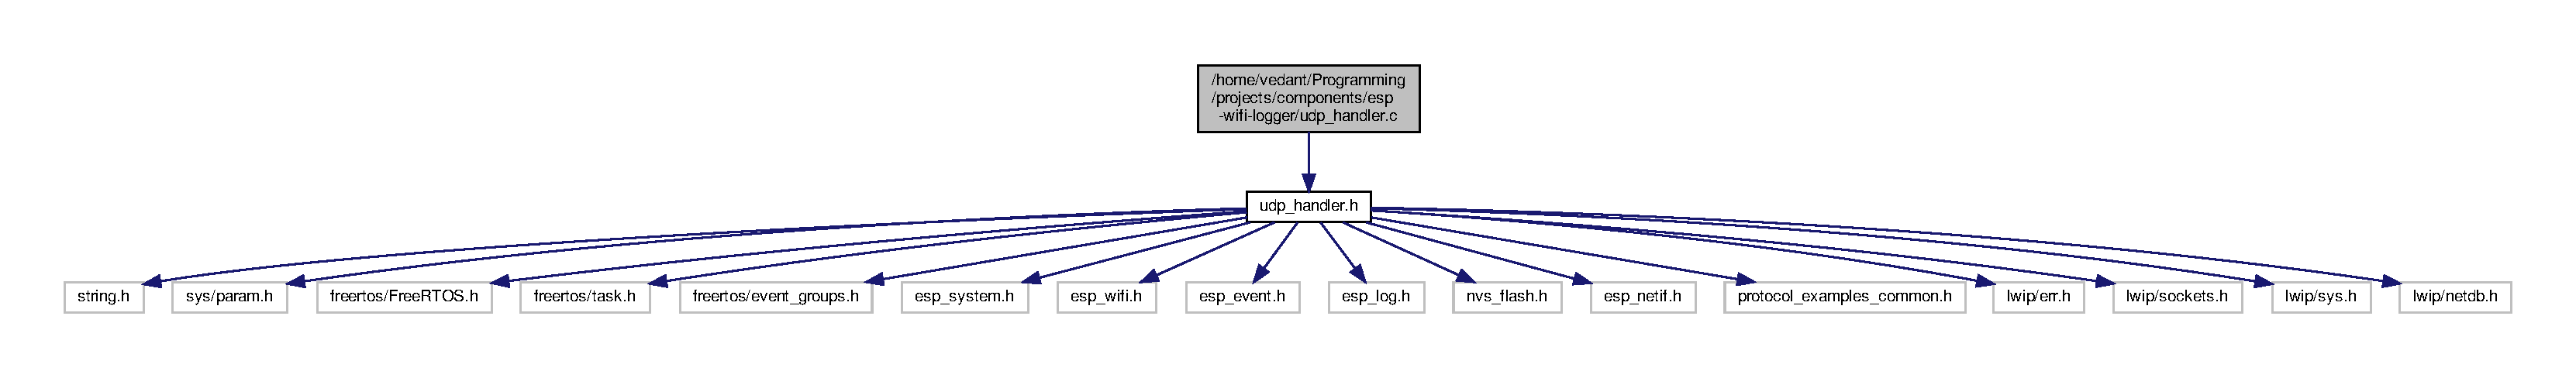
\includegraphics[width=350pt]{udp__handler_8c__incl}
\end{center}
\end{figure}
\subsection*{Functions}
\begin{DoxyCompactItemize}
\item 
void \hyperlink{udp__handler_8c_a412aa3402fc47e327861b48a04c3c08a}{network\+\_\+manager} (struct \hyperlink{structnetwork__data}{network\+\_\+data} $\ast$nm)
\begin{DoxyCompactList}\small\item\em Manages U\+DP connection to the server. \end{DoxyCompactList}\item 
int \hyperlink{udp__handler_8c_a7ddbd791c1d13c96db95eba36aae6145}{send\+\_\+data} (struct \hyperlink{structnetwork__data}{network\+\_\+data} $\ast$nm, char $\ast$payload)
\begin{DoxyCompactList}\small\item\em Sends data to the server through a U\+DP socket. \end{DoxyCompactList}\item 
char $\ast$ \hyperlink{udp__handler_8c_afe419fdd19f7194dcf9c9e6d00118224}{recieve\+\_\+data} (struct \hyperlink{structnetwork__data}{network\+\_\+data} $\ast$nm)
\begin{DoxyCompactList}\small\item\em Receives data from U\+DP server. \end{DoxyCompactList}\item 
void \hyperlink{udp__handler_8c_a3e138ed94c89bd74c249c9f4a1a4c642}{close\+\_\+network\+\_\+manager} (struct \hyperlink{structnetwork__data}{network\+\_\+data} $\ast$nm)
\begin{DoxyCompactList}\small\item\em Shutdown active connection, deallocate memory. \end{DoxyCompactList}\end{DoxyCompactItemize}


\subsection{Function Documentation}
\mbox{\Hypertarget{udp__handler_8c_a3e138ed94c89bd74c249c9f4a1a4c642}\label{udp__handler_8c_a3e138ed94c89bd74c249c9f4a1a4c642}} 
\index{udp\+\_\+handler.\+c@{udp\+\_\+handler.\+c}!close\+\_\+network\+\_\+manager@{close\+\_\+network\+\_\+manager}}
\index{close\+\_\+network\+\_\+manager@{close\+\_\+network\+\_\+manager}!udp\+\_\+handler.\+c@{udp\+\_\+handler.\+c}}
\subsubsection{\texorpdfstring{close\+\_\+network\+\_\+manager()}{close\_network\_manager()}}
{\footnotesize\ttfamily void close\+\_\+network\+\_\+manager (\begin{DoxyParamCaption}\item[{struct \hyperlink{structnetwork__data}{network\+\_\+data} $\ast$}]{nm }\end{DoxyParamCaption})}



Shutdown active connection, deallocate memory. 


\begin{DoxyParams}{Parameters}
{\em nm} & \hyperlink{structtcp__network__data}{tcp\+\_\+network\+\_\+data} struct which contains connection info \\
\hline
\end{DoxyParams}
\begin{DoxyReturn}{Returns}
void 
\end{DoxyReturn}
\mbox{\Hypertarget{udp__handler_8c_a412aa3402fc47e327861b48a04c3c08a}\label{udp__handler_8c_a412aa3402fc47e327861b48a04c3c08a}} 
\index{udp\+\_\+handler.\+c@{udp\+\_\+handler.\+c}!network\+\_\+manager@{network\+\_\+manager}}
\index{network\+\_\+manager@{network\+\_\+manager}!udp\+\_\+handler.\+c@{udp\+\_\+handler.\+c}}
\subsubsection{\texorpdfstring{network\+\_\+manager()}{network\_manager()}}
{\footnotesize\ttfamily void network\+\_\+manager (\begin{DoxyParamCaption}\item[{struct \hyperlink{structnetwork__data}{network\+\_\+data} $\ast$}]{nm }\end{DoxyParamCaption})}



Manages U\+DP connection to the server. 


\begin{DoxyParams}{Parameters}
{\em nm} & \hyperlink{structnetwork__data}{network\+\_\+data} struct which contains necessary data for a U\+DP connection \\
\hline
\end{DoxyParams}
\begin{DoxyReturn}{Returns}
void 
\end{DoxyReturn}
\mbox{\Hypertarget{udp__handler_8c_afe419fdd19f7194dcf9c9e6d00118224}\label{udp__handler_8c_afe419fdd19f7194dcf9c9e6d00118224}} 
\index{udp\+\_\+handler.\+c@{udp\+\_\+handler.\+c}!recieve\+\_\+data@{recieve\+\_\+data}}
\index{recieve\+\_\+data@{recieve\+\_\+data}!udp\+\_\+handler.\+c@{udp\+\_\+handler.\+c}}
\subsubsection{\texorpdfstring{recieve\+\_\+data()}{recieve\_data()}}
{\footnotesize\ttfamily char$\ast$ recieve\+\_\+data (\begin{DoxyParamCaption}\item[{struct \hyperlink{structnetwork__data}{network\+\_\+data} $\ast$}]{nm }\end{DoxyParamCaption})}



Receives data from U\+DP server. 


\begin{DoxyParams}{Parameters}
{\em nm} & \hyperlink{structnetwork__data}{network\+\_\+data} struct which contains connection info \\
\hline
\end{DoxyParams}
\begin{DoxyReturn}{Returns}
char array which contains data received 
\end{DoxyReturn}
\mbox{\Hypertarget{udp__handler_8c_a7ddbd791c1d13c96db95eba36aae6145}\label{udp__handler_8c_a7ddbd791c1d13c96db95eba36aae6145}} 
\index{udp\+\_\+handler.\+c@{udp\+\_\+handler.\+c}!send\+\_\+data@{send\+\_\+data}}
\index{send\+\_\+data@{send\+\_\+data}!udp\+\_\+handler.\+c@{udp\+\_\+handler.\+c}}
\subsubsection{\texorpdfstring{send\+\_\+data()}{send\_data()}}
{\footnotesize\ttfamily int send\+\_\+data (\begin{DoxyParamCaption}\item[{struct \hyperlink{structnetwork__data}{network\+\_\+data} $\ast$}]{nm,  }\item[{char $\ast$}]{payload }\end{DoxyParamCaption})}



Sends data to the server through a U\+DP socket. 


\begin{DoxyParams}{Parameters}
{\em nm} & A pointer to \hyperlink{structnetwork__data}{network\+\_\+data} struct \\
\hline
{\em payload} & char array which contains data to be sent \\
\hline
\end{DoxyParams}
\begin{DoxyReturn}{Returns}
int -\/ returns -\/1 if sending failed, number of bytes sent if successfully sent the data 
\end{DoxyReturn}

\hypertarget{utils_8cpp}{}\section{/home/vedant/\+Programming/projects/components/esp-\/wifi-\/logger/utils.cpp File Reference}
\label{utils_8cpp}\index{/home/vedant/\+Programming/projects/components/esp-\/wifi-\/logger/utils.\+cpp@{/home/vedant/\+Programming/projects/components/esp-\/wifi-\/logger/utils.\+cpp}}
{\ttfamily \#include \char`\"{}utils.\+h\char`\"{}}\newline
Include dependency graph for utils.\+cpp\+:\nopagebreak
\begin{figure}[H]
\begin{center}
\leavevmode
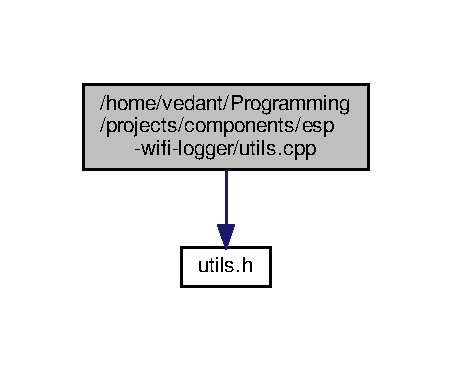
\includegraphics[width=217pt]{utils_8cpp__incl}
\end{center}
\end{figure}
\subsection*{Functions}
\begin{DoxyCompactItemize}
\item 
char $\ast$ \hyperlink{utils_8cpp_af768902cbc75dc282b88515dd045b7b5}{generate\+\_\+log\+\_\+message\+\_\+timestamp} (uint32\+\_\+t timestamp, char $\ast$log\+\_\+message)
\begin{DoxyCompactList}\small\item\em adds timestamp to the log message \end{DoxyCompactList}\end{DoxyCompactItemize}


\subsection{Function Documentation}
\mbox{\Hypertarget{utils_8cpp_af768902cbc75dc282b88515dd045b7b5}\label{utils_8cpp_af768902cbc75dc282b88515dd045b7b5}} 
\index{utils.\+cpp@{utils.\+cpp}!generate\+\_\+log\+\_\+message\+\_\+timestamp@{generate\+\_\+log\+\_\+message\+\_\+timestamp}}
\index{generate\+\_\+log\+\_\+message\+\_\+timestamp@{generate\+\_\+log\+\_\+message\+\_\+timestamp}!utils.\+cpp@{utils.\+cpp}}
\subsubsection{\texorpdfstring{generate\+\_\+log\+\_\+message\+\_\+timestamp()}{generate\_log\_message\_timestamp()}}
{\footnotesize\ttfamily char$\ast$ generate\+\_\+log\+\_\+message\+\_\+timestamp (\begin{DoxyParamCaption}\item[{uint32\+\_\+t}]{timestamp,  }\item[{char $\ast$}]{log\+\_\+message }\end{DoxyParamCaption})}



adds timestamp to the log message 


\begin{DoxyParams}{Parameters}
{\em timestamp} & timestamp provided by E\+SP in milliseconds \\
\hline
{\em log\+\_\+message} & log message to be sent through wifi \\
\hline
\end{DoxyParams}
\begin{DoxyReturn}{Returns}
char$\ast$ final log message with timestamp 
\end{DoxyReturn}

\hypertarget{wifi__logger_8c}{}\section{/home/vedant/\+Programming/projects/components/esp-\/wifi-\/logger/wifi\+\_\+logger.c File Reference}
\label{wifi__logger_8c}\index{/home/vedant/\+Programming/projects/components/esp-\/wifi-\/logger/wifi\+\_\+logger.\+c@{/home/vedant/\+Programming/projects/components/esp-\/wifi-\/logger/wifi\+\_\+logger.\+c}}
{\ttfamily \#include \char`\"{}wifi\+\_\+logger.\+h\char`\"{}}\newline
Include dependency graph for wifi\+\_\+logger.\+c\+:\nopagebreak
\begin{figure}[H]
\begin{center}
\leavevmode
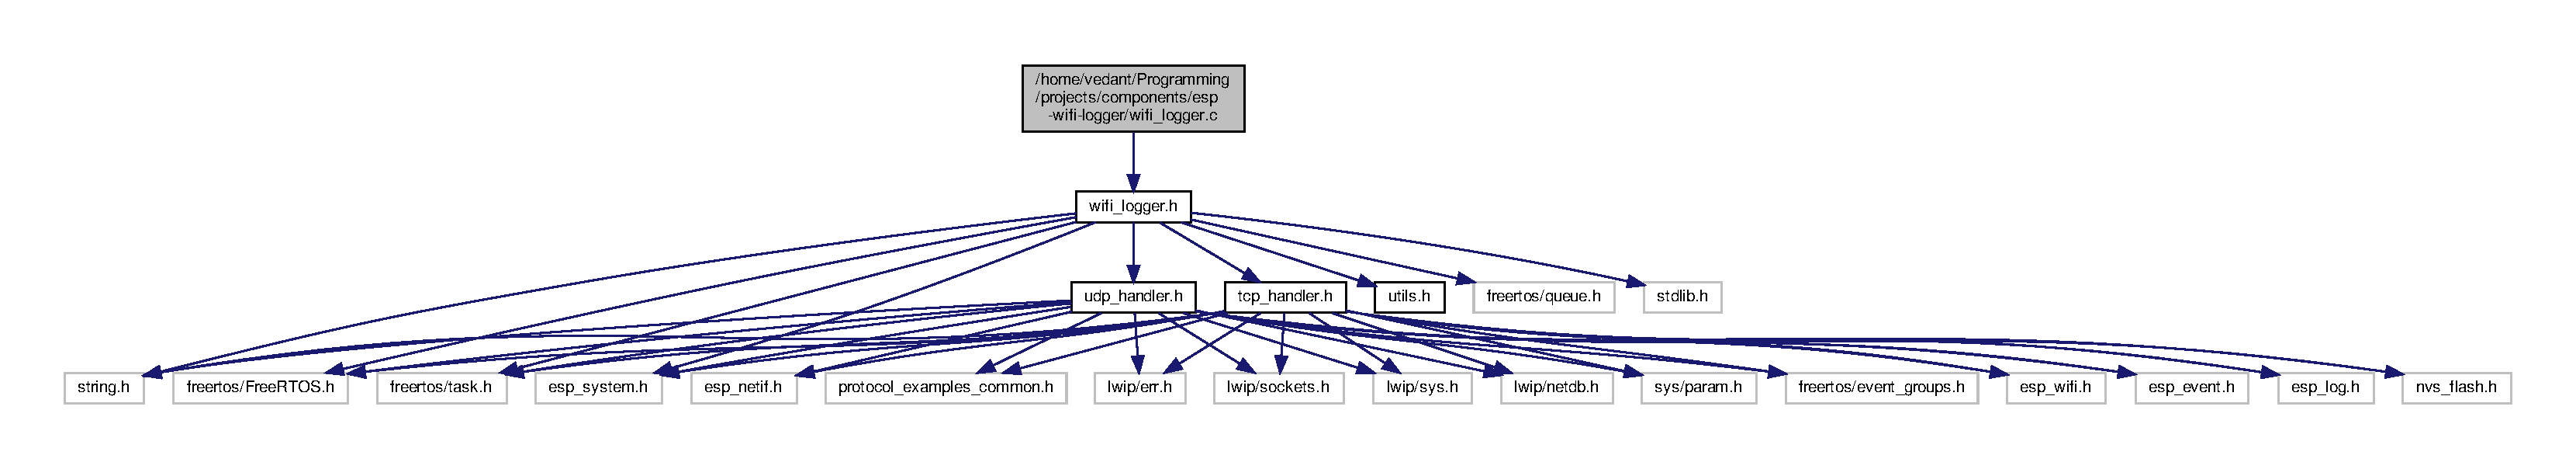
\includegraphics[width=350pt]{wifi__logger_8c__incl}
\end{center}
\end{figure}
\subsection*{Functions}
\begin{DoxyCompactItemize}
\item 
esp\+\_\+err\+\_\+t \hyperlink{wifi__logger_8c_a320afeaba56579760e7e3185a3d1fa02}{init\+\_\+queue} (void)
\begin{DoxyCompactList}\small\item\em Initialises message queue. \end{DoxyCompactList}\item 
void \hyperlink{wifi__logger_8c_aea5e8c4231b83bde5f8f0f4556271aba}{init\+\_\+wifi} (void)
\begin{DoxyCompactList}\small\item\em Initialises and connects to wifi. \end{DoxyCompactList}\item 
esp\+\_\+err\+\_\+t \hyperlink{wifi__logger_8c_a2261c877b2e047a36b7df77259b689ec}{send\+\_\+to\+\_\+queue} (const char $\ast$log\+\_\+message)
\begin{DoxyCompactList}\small\item\em Sends log message to message queue. \end{DoxyCompactList}\item 
char $\ast$ \hyperlink{wifi__logger_8c_ad28af408449f666a77441f0120a6a228}{receive\+\_\+from\+\_\+queue} (void)
\begin{DoxyCompactList}\small\item\em Receive data from queue. \end{DoxyCompactList}\item 
void \hyperlink{wifi__logger_8c_a479c62eb886c1c0aa898a033916bb653}{generate\+\_\+log\+\_\+message} (const char $\ast$T\+AG, int line, const char $\ast$func, const char $\ast$fmt,...)
\begin{DoxyCompactList}\small\item\em generates log message, of the format generated by E\+S\+P\+\_\+\+L\+OG function \end{DoxyCompactList}\item 
void \hyperlink{wifi__logger_8c_a8e612786031d82bb0eac8affe469ed2c}{start\+\_\+wifi\+\_\+logger} (void)
\begin{DoxyCompactList}\small\item\em wrapper function to start wifi logger \end{DoxyCompactList}\end{DoxyCompactItemize}


\subsection{Function Documentation}
\mbox{\Hypertarget{wifi__logger_8c_a479c62eb886c1c0aa898a033916bb653}\label{wifi__logger_8c_a479c62eb886c1c0aa898a033916bb653}} 
\index{wifi\+\_\+logger.\+c@{wifi\+\_\+logger.\+c}!generate\+\_\+log\+\_\+message@{generate\+\_\+log\+\_\+message}}
\index{generate\+\_\+log\+\_\+message@{generate\+\_\+log\+\_\+message}!wifi\+\_\+logger.\+c@{wifi\+\_\+logger.\+c}}
\subsubsection{\texorpdfstring{generate\+\_\+log\+\_\+message()}{generate\_log\_message()}}
{\footnotesize\ttfamily void generate\+\_\+log\+\_\+message (\begin{DoxyParamCaption}\item[{const char $\ast$}]{T\+AG,  }\item[{int}]{line,  }\item[{const char $\ast$}]{func,  }\item[{const char $\ast$}]{fmt,  }\item[{}]{... }\end{DoxyParamCaption})}



generates log message, of the format generated by E\+S\+P\+\_\+\+L\+OG function 


\begin{DoxyParams}{Parameters}
{\em T\+AG} & Tag for the log message \\
\hline
{\em line} & line \\
\hline
{\em func} & func \\
\hline
{\em fmt} & fmt \\
\hline
\end{DoxyParams}
\mbox{\Hypertarget{wifi__logger_8c_a320afeaba56579760e7e3185a3d1fa02}\label{wifi__logger_8c_a320afeaba56579760e7e3185a3d1fa02}} 
\index{wifi\+\_\+logger.\+c@{wifi\+\_\+logger.\+c}!init\+\_\+queue@{init\+\_\+queue}}
\index{init\+\_\+queue@{init\+\_\+queue}!wifi\+\_\+logger.\+c@{wifi\+\_\+logger.\+c}}
\subsubsection{\texorpdfstring{init\+\_\+queue()}{init\_queue()}}
{\footnotesize\ttfamily esp\+\_\+err\+\_\+t init\+\_\+queue (\begin{DoxyParamCaption}\item[{void}]{ }\end{DoxyParamCaption})}



Initialises message queue. 

\begin{DoxyReturn}{Returns}
esp\+\_\+err\+\_\+t E\+S\+P\+\_\+\+OK -\/ if queue init sucessfully, E\+S\+P\+\_\+\+F\+A\+IL -\/ if queue init failed 
\end{DoxyReturn}
\mbox{\Hypertarget{wifi__logger_8c_aea5e8c4231b83bde5f8f0f4556271aba}\label{wifi__logger_8c_aea5e8c4231b83bde5f8f0f4556271aba}} 
\index{wifi\+\_\+logger.\+c@{wifi\+\_\+logger.\+c}!init\+\_\+wifi@{init\+\_\+wifi}}
\index{init\+\_\+wifi@{init\+\_\+wifi}!wifi\+\_\+logger.\+c@{wifi\+\_\+logger.\+c}}
\subsubsection{\texorpdfstring{init\+\_\+wifi()}{init\_wifi()}}
{\footnotesize\ttfamily void init\+\_\+wifi (\begin{DoxyParamCaption}\item[{void}]{ }\end{DoxyParamCaption})}



Initialises and connects to wifi. 

\mbox{\Hypertarget{wifi__logger_8c_ad28af408449f666a77441f0120a6a228}\label{wifi__logger_8c_ad28af408449f666a77441f0120a6a228}} 
\index{wifi\+\_\+logger.\+c@{wifi\+\_\+logger.\+c}!receive\+\_\+from\+\_\+queue@{receive\+\_\+from\+\_\+queue}}
\index{receive\+\_\+from\+\_\+queue@{receive\+\_\+from\+\_\+queue}!wifi\+\_\+logger.\+c@{wifi\+\_\+logger.\+c}}
\subsubsection{\texorpdfstring{receive\+\_\+from\+\_\+queue()}{receive\_from\_queue()}}
{\footnotesize\ttfamily char$\ast$ receive\+\_\+from\+\_\+queue (\begin{DoxyParamCaption}\item[{void}]{ }\end{DoxyParamCaption})}



Receive data from queue. 

\begin{DoxyReturn}{Returns}
char$\ast$ -\/ returns log message received from the queue, returns N\+U\+LL if error or timeout 
\end{DoxyReturn}
\mbox{\Hypertarget{wifi__logger_8c_a2261c877b2e047a36b7df77259b689ec}\label{wifi__logger_8c_a2261c877b2e047a36b7df77259b689ec}} 
\index{wifi\+\_\+logger.\+c@{wifi\+\_\+logger.\+c}!send\+\_\+to\+\_\+queue@{send\+\_\+to\+\_\+queue}}
\index{send\+\_\+to\+\_\+queue@{send\+\_\+to\+\_\+queue}!wifi\+\_\+logger.\+c@{wifi\+\_\+logger.\+c}}
\subsubsection{\texorpdfstring{send\+\_\+to\+\_\+queue()}{send\_to\_queue()}}
{\footnotesize\ttfamily esp\+\_\+err\+\_\+t send\+\_\+to\+\_\+queue (\begin{DoxyParamCaption}\item[{const char $\ast$}]{log\+\_\+message }\end{DoxyParamCaption})}



Sends log message to message queue. 


\begin{DoxyParams}{Parameters}
{\em log\+\_\+message} & log message to be sent to the queue \\
\hline
\end{DoxyParams}
\begin{DoxyReturn}{Returns}
esp\+\_\+err\+\_\+t E\+S\+P\+\_\+\+OK -\/ if queue init sucessfully, E\+S\+P\+\_\+\+F\+A\+IL -\/ if queue init failed 
\end{DoxyReturn}
\mbox{\Hypertarget{wifi__logger_8c_a8e612786031d82bb0eac8affe469ed2c}\label{wifi__logger_8c_a8e612786031d82bb0eac8affe469ed2c}} 
\index{wifi\+\_\+logger.\+c@{wifi\+\_\+logger.\+c}!start\+\_\+wifi\+\_\+logger@{start\+\_\+wifi\+\_\+logger}}
\index{start\+\_\+wifi\+\_\+logger@{start\+\_\+wifi\+\_\+logger}!wifi\+\_\+logger.\+c@{wifi\+\_\+logger.\+c}}
\subsubsection{\texorpdfstring{start\+\_\+wifi\+\_\+logger()}{start\_wifi\_logger()}}
{\footnotesize\ttfamily void start\+\_\+wifi\+\_\+logger (\begin{DoxyParamCaption}\item[{void}]{ }\end{DoxyParamCaption})}



wrapper function to start wifi logger 


%--- End generated contents ---

% Index
\backmatter
\newpage
\phantomsection
\clearemptydoublepage
\addcontentsline{toc}{chapter}{Index}
\printindex

\end{document}
